\documentclass{article}
\usepackage{listings}
\usepackage{color}
\usepackage{url}
\usepackage{graphicx}
\usepackage{titlesec}
\usepackage{wrapfig}
\usepackage{tabularx}
\usepackage{dirtree}
\usepackage{xcolor}
\usepackage{floatrow}

\setcounter{secnumdepth}{4}

\titleformat{\paragraph}
{\normalfont\normalsize\bfseries}{\theparagraph}{1em}{}
\titlespacing*{\paragraph}
{0pt}{3.25ex plus 1ex minus .2ex}{1.5ex plus .2ex}

% Define colors
\definecolor{codegreen}{rgb}{0,0.6,0}
\definecolor{codegray}{rgb}{0.5,0.5,0.5}
\definecolor{codepurple}{rgb}{0.58,0,0.82}
\definecolor{backcolour}{rgb}{0.95,0.95,0.92}

% Define global lstlisting settings
\lstset{
    language=C, % Change this to the desired language
    basicstyle=\small\ttfamily, % Set the basic font style and size
    numbers=left, % Display line numbers on the left
    numberstyle=\tiny\color{codegray}, % Set the line number style
    stepnumber=1, % Set the step between line numbers
    numbersep=5pt, % Set the distance between line numbers and code
    backgroundcolor=\color{backcolour}, % Set the background color
    showspaces=false, % Don't show spaces in strings
    showstringspaces=false, % Don't show spaces in strings as special characters
    showtabs=false, % Don't show tabs as special characters
    tabsize=4, % Set the tab size
    captionpos=b, % Set the caption position at the bottom
    breaklines=true, % Wrap long lines
    breakatwhitespace=true, % Wrap at whitespace
    escapeinside={\%*}{*)}, % Add LaTeX code within your code
    morekeywords={*,...}, % Add more keywords if necessary
}

\title{Exercise Tracker Website \\ \vspace{10pt} \large Computer Science A-Level Project \normalsize}
\author{Marcus Ciobanu}
\date{}

\begin{document}

\maketitle
\newpage

\tableofcontents
\newpage

\section{Citations}
Listed in order of their appearance:
\begin{itemize}
  \item Statista (2022). UK fitness/health club market size 2021 | Statista. [online] Statista. Available at: \url{https://www.statista.com/statistics/1194831/fitness-health-club-market-size-uk/}.
  \item MDN Web Docs. (n.d.). Django introduction. [online] Available at: \url{https://developer.mozilla.org/en-US/docs/Learn/Server-side/Django/Introduction.}
\end{itemize}
\newpage

\section{Analysis}

\subsection{Define the Problem}
In recent years, the fitness industry has seen a boom in revenue and participation, with more people than ever being conscious of their health and diet. The figure below shows the market size of the gym, health \& fitness clubs industry in the United Kingdom (UK) from 2012 to 2022. As can be seen, there has been a steady increase up until 2020. 

Following this point, the COVID-19 pandemic caused a major blow to the gym industry. However, this is not representative of fitness as a whole. What the pandemic actually caused was a huge influx of beginners to fitness who, as a result of their abundance of free time and boredom, took up exercise. Furthermore, the figure also indicates a huge gain in market size from 2021 to 2022 as gyms opened back up. It can be expected that this trend will continue and the fitness industry’s market share will soar to new heights as those who began exercising during the pandemic purchase gym memberships.
\begin{figure}[ht]
  \raggedright
  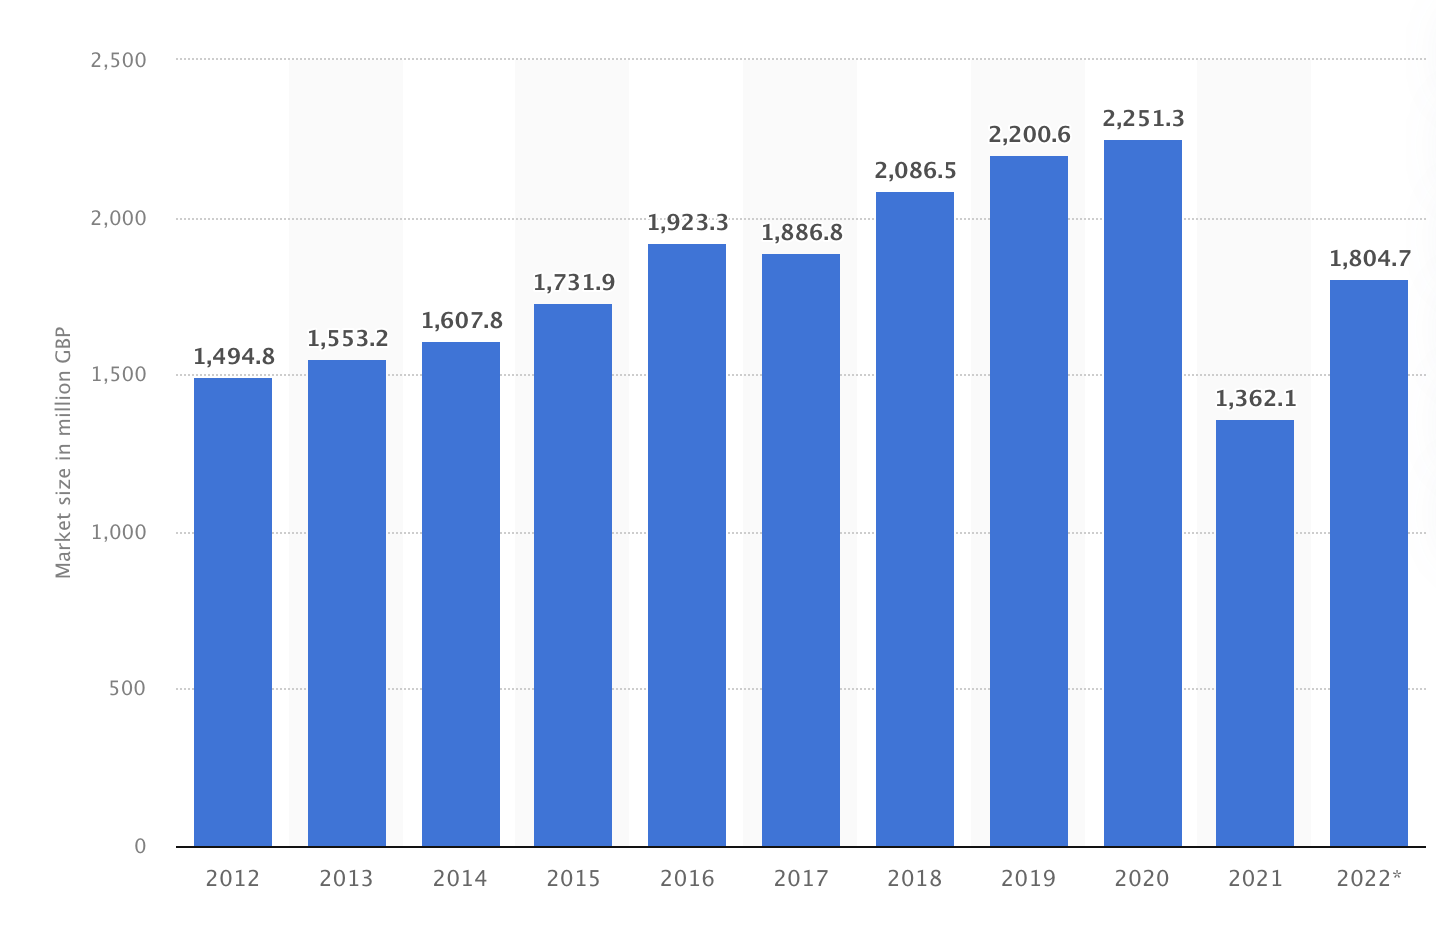
\includegraphics[width=1\textwidth]{Figure 1.png}
  \caption{Industry market size}
  \label{fig:Figure 1}
\end{figure}

As a result of the growth of the market, there is now room for competition in the digital fitness space(a previously monopolised industry where major players held the majority of the user base). New developments have the opportunity to seize user attention by solving their problems and capitalising on the unique needs of beginners.

From my own previous experience as a beginner in fitness, I can attest to the difficulty and friction associated with trying to record down everything manually. Having to carry a notebook and pen to every session is cumbersome and the formatting is often inconsistent. For the modern gym-goer, it is important to have a solution to this problem. The reason for tracking progress in the first place is that it is a critical element in optimising results to build muscle and/or lose weight. Rep ranges must be tracked and weight on the bar must be carefully monitored to maximise results for the minimum amount of effort. Evidently, such an endeavour is complex by nature, hence the need to make this as smooth and easy as possible for the beginner (lest they become demotivated and give up altogether). After all, if the experience is frictionless then you are more likely to record down all your workouts, leading to higher consistency and better results due to the compounding nature of incremental progress. 

In summary, there are more beginners than ever in fitness. Beginners suffer from a lack of knowledge regarding what to do. A simple solution that is easy and frictionless is required to help them track their activities and maximise progress. Therefore, my programming project involves developing an exercise tracking website that makes this process seamless and intuitive. 

\subsection{Why the Problem is suited to a Computational Solution}
Much of the suitability for this problem being suited to a computational solution stems from why this is a problem in the first place. Simply put, the analogue equivalent is massively inferior to any variation of a digital solution and makes it difficult for people to stick to it which harms progress. There are multiple reasons for this:
\begin{enumerate}
  \item As you advance, you will reach the point of having done hundreds of workouts. This results in thousands of exercises, tens of thousands of sets and hundreds of thousands of reps. Therefore, this large volume of data is best suited to being kept digitally, as it would result in many pages if done in analogue form.
  \item Pages are liable to physical damage such as being lost or set on fire, this is a risk as it could mean that you are unable to see what you have done previously or track your progress over an extended period of time. In contrast, data can be backed up on the cloud when done digitally, meaning it is kept safe.
  \item Handwriting can often be untidy and unclear and takes longer than typing or entering values into a database interface digitally. 
  \item Pages cannot be easily sorted through to gather meaningful insights (producing graphs for example) and could be sped up and made far more efficient through use of algorithms and computing power. 
  \item You do not need to bring a pen and paper to the gym with you if it is done digitally, as it can all be done on your phone which most people bring everywhere with them regardless. 
\end{enumerate}
\subsubsection{Computational methods that are appropriate}
As well as the reasons listed above that focus more on the comparison between the digital and analogue ways of solving the problem, there are also computational methods and constructs that lend themselves to the efficient and streamlined solving of the problem.
\paragraph{Thinking abstractly}
For in depth analysis and generation of insights from the data the user records such as producing graphs that display progress in a certain lift over time, abstraction can be used. The mechanisms behind the production of the graph are abstracted from the user for maximum ease of use and pure functionality. 

They would simply record their results into a GUI and select the option to produce a graph, much like how a programmer can input parameters into a function imported from a library. They know what it does and what is required to make it produce the results but do not and do not need to understand how it works. If we were to contrast this to the analogue equivalent, the user would need to understand how to plot graphs and translate data into the necessary formats. In this case, the use of abstraction not only lends itself to the computational solution but enhances it.
\paragraph{Thinking ahead}
Through the use of a computational solution, we can identify recurring scenarios and therefore develop functions that can be reused every time the user wants to carry out that task. For example, we know that if the user is using an exercise tracker they are going to want to record many workouts. Therefore, we can produce functions that take the expected inputs for these tasks (sets, reps, etc.) and produce outputs in a consistent, comparable format.
\newpage
\paragraph{Thinking procedurally}
\begin{wrapfigure}{l}{0.2\textwidth} % 'l' for left side, and width of the wrap
  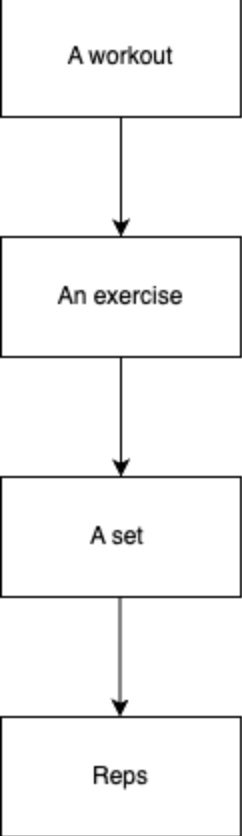
\includegraphics[width=0.2\textwidth]{Figure 2.png}
  \caption{Top-down design}
\end{wrapfigure}
When a user performs a workout, we understand that there will be a set ‘formula’ which they follow each time in a procedural manner. They would typically select an exercise, create a set then perform the reps that make up that set. Therefore, we can model this within the code through the use of a top-down design. 

As can be seen in the figure, we can break down the idea of a workout into nested modules of code in an order that the user would typically think of it in. These modules can then communicate with each other along the chain to produce the desired output. 

This method of top-design and decomposition is not only natural to the way of thinking of the user, but is also computationally efficient and speeds up the development process. It will also make the program far easier to maintain and test due to its modular nature. 

The modular nature also relates to thinking ahead, as it promotes code reusability and applying the same code to multiple iterations of the same scenario, further decreasing development time needed whilst ensuring consistent formatting and familiarity to the user. 

\subsection{Stakeholders}
Naturally, the primary group of stakeholders will be hobbyist gym goers, mostly due to the fact that they make up the majority of consumers in the market. Therefore, the website will be tailored to suit the needs of beginners to intermediates to maximise the usefulness to the average user. For example, all the exercises in the exercise database will include explanations on how to perform the exercise and what muscle groups it trains. Another example is the goal setting feature that will be included in the signup process which generates a recommended goal for them based on the information they enter during signup. Regardless, there will still be many features applicable to more advanced users as well, as the crossover is substantial and the core features of the website have utility throughout the spectrum of users.

The software is not intended for use by people under the age of 16, as this is the typical age requirement for most gyms and so it would be a poor use of resources and development time to make considerations for this user group. Despite this, the program is still usable by this group and there is no hard restriction in place to prevent them from using it. Simply put, it will not be designed in a way that places any priority on their specific needs and use cases, but they may be able to still use it for home workouts involving callisthenics and other bodyweight movements that do not require a gym to perform. 

In terms of people with disabilities, both mental and physical, the program retains its utility. Furthermore, no special features need be designed to cater for them. For anyone with physical disabilities, they can simply select the exercises that they can perform safely and to a good standard with their own disability in mind. Many exercises can be performed without the use of legs, for example dumbbell hammer curls. Therefore, in this case, the user will make their own adjustments so that the program can suit their needs. For anyone with mental disabilities, this should not have much impact on their ability to perform exercises, so the program should work as intended for them. However, the program will not cater for anyone with impaired vision, due to the difficulty of development of a comprehensive audio navigation system. This is a limitation, and restricts the user base for the project. 

Here is an example stakeholder to illustrate a typical use case:

\begin{figure}[ht]
  \centering
  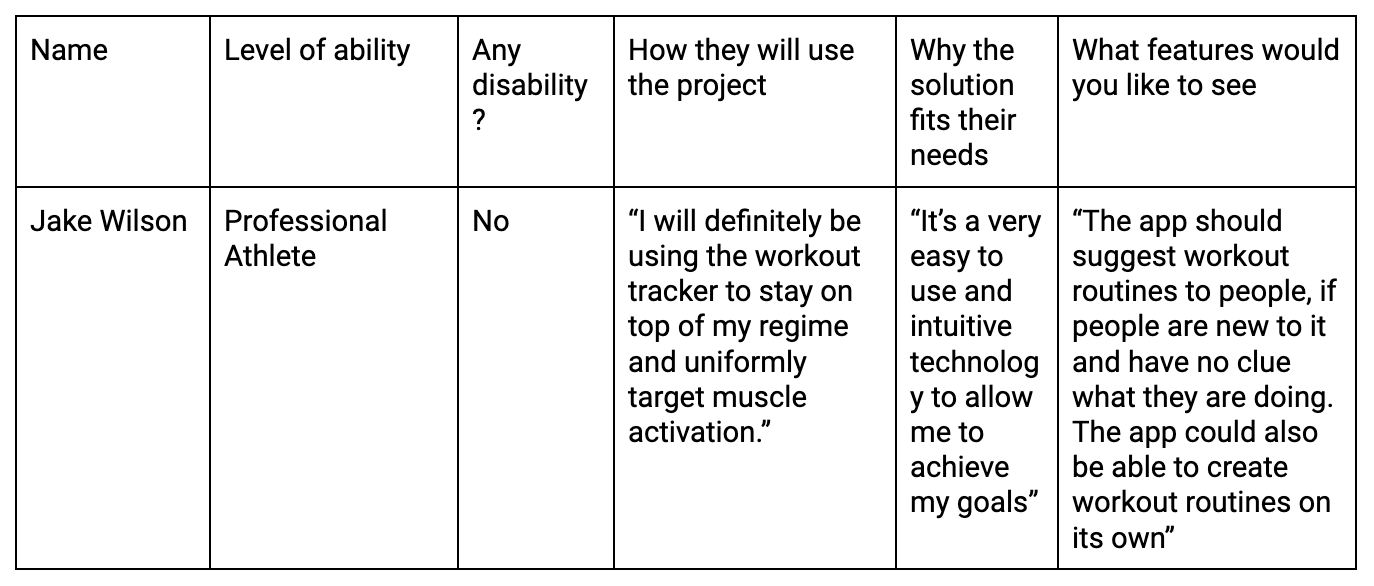
\includegraphics[width=1\textwidth]{Figure 3.png}
  \caption{Example stakeholder}
\end{figure}

Utilising feedback and requests from potential stakeholders such as Jake will be vital in ensuring that the finished project meets the needs and requirements of those who will be most likely to use it.

This iterative process of feedback and adjustment is important to increase customer satisfaction and widen the user base however it is also important to place limitations on what is realistic and achievable in the timeframe as what is just as important to stakeholders as a feature rich program is that the program is delivered on time and within budget. The balance between these two elements is something that will remain in mind throughout the whole project. 

\subsection{Research}

\subsubsection{Existing Systems}
There are two major existing systems that offer a workout tracking system similar to the proposed solution. These are Hevy and Strong. Alongside the research that follows, I have been a user of both programs at separate times for over a year so I believe this first-hand experience with both gives me the necessary insight to properly evaluate their features and identify the correct way to take on board this information for my own project. 

\paragraph{Hevy}
Hevy is the premier workout tracking app on the Android Play Store. The platform is different to the proposed solution (mobile vs. browser) but the core features remain the same and so it is valid to analyse. It incorporates workout tracking with a social media system where you can follow others and share your workouts and progress with a following. It works sort of like Instagram in that regard, being able to like and comment on others workouts. However, this element of the program is completely optional as you can make your account private, so for the purpose of this research, I will not be looking at this element of the program. It is also the cheaper of the 2 existing solutions priced at £2.99/month compared to Strong which is £4.69/month. 

\begin{figure}[H]
  \centering
  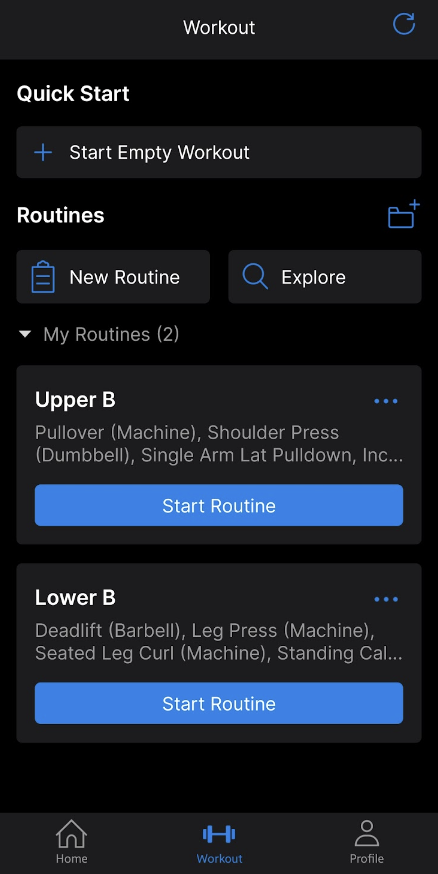
\includegraphics[width=0.4\textwidth]{Figure 4.png}
  \caption{Quick start page}
\end{figure}

The general consensus among users is that Hevy offers more features for analysis and tracking for a cheaper price whilst Strong offers a slick, clean UI with the actual workout tracking part of the app being very intuitive and easy to use. However, this is all subjective and in terms of user ratings, they both sit at a high 4 star rating with minimal criticism of either application.

In the surrounding pages are a few screenshots from my mobile phone from the app which illustrate a few key features that I will go through and evaluate. They cover a range of the app’s features from its workout tracking capabilities to its extensive section for analysis of progress and workouts. 

See Figure 4, the main section of the application which allows you to record your workouts. You can either create your own routines, choose from a range of templates in the explore section or select the quick start option. This will allow you to go straight into a workout and add your exercises on the fly. 

There is also an option to create routine folders. This allows increased organisation and to periodise your training into blocks sorted by folder (a useful feature for more advanced lifters who may want to alternate between load and deload periods). This could definitely be a feature to adopt in order to ensure that the program has adequate tailoring for all ability ranges. 

\begin{figure}[H]
  \centering
  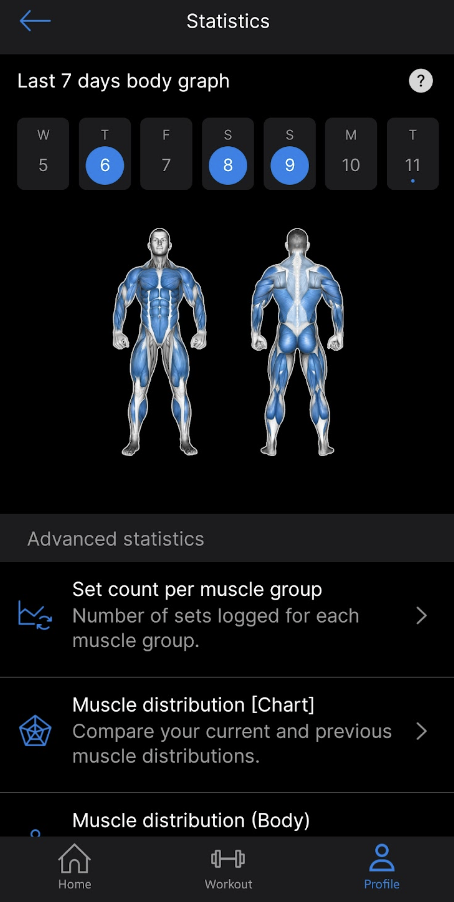
\includegraphics[width=0.4\textwidth]{Figure 5.png}
  \caption{Statistics page}
\end{figure}

Overall, Hevy does a great job of offering options for all use cases and ability levels, with customizability available if needed but not required. Furthermore, the UI is slick and intuitive, which is necessary for a small mobile screen.

The statistics section of the application is rather unique to Hevy, where you can analyse your progress in as much detail as you want to aid in organisation and planning. In particular, the heatmap is very useful, allowing you to see at a glance which muscle groups you have hit during that week. You can therefore quickly identify lacking muscles and pick exercises for your next workout that target them specifically. 

The advanced statistics section allows for a more indepth look at what the heatmap gives you at a glance. It logs sets per muscle group and shows a spider web chart of the distribution. All of these features can be leveraged for increased control and data on your progress. However, all of this is optional and doesn’t need to be used which is a good feature of
Hevy. It is as in depth and detailed as you want it to be.

\begin{figure}[H]
  \centering
  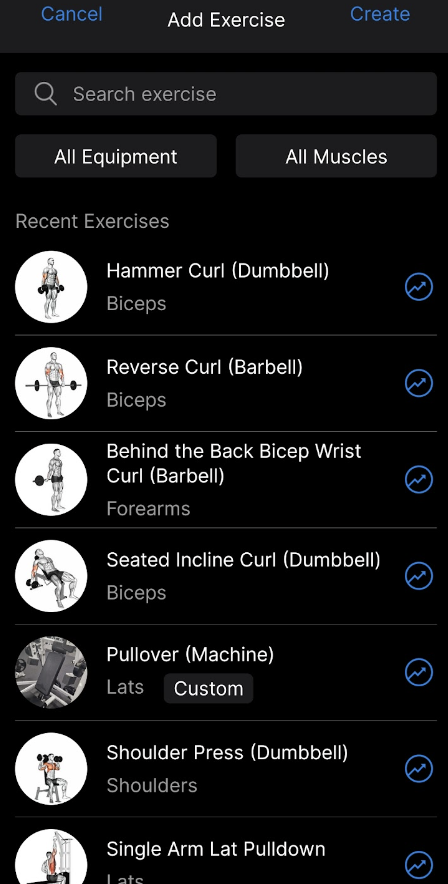
\includegraphics[width=0.4\textwidth]{Figure 6.png}
  \caption{Add exercise page}
\end{figure}

Figure 6 shows the exercise addition menu once you either start a routine or start empty exercise.

There is a large bank of premade exercises that cover nearly everything you will need. They also include an image and sometimes a video with instructions explaining how to perform every exercise. This is undoubtedly useful for beginners but more advanced lifters may want to do further research to optimise form and technique. 

All exercises when selected are automatically logged into a database, as well as the sets and reps you will go on to perform. 

As you can see further down the list, there is an exercise called ‘Pullover (Machine)’. This is a custom exercise. You can create your own exercises if your gym has some niche machinery or you wish to perform uncommon variations of certain exercises that cannot be found in the premade exercises. 

See Figure 7, this is the exercise creation menu. It can be accessed from the exercise addition menu by clicking on the button in the top right. 

You can create any exercise possible due to the features of the creation menu. A custom name and picture can be given. More importantly, the muscles it targets (both primary and secondary) are included, as well as the exercise type and equipment. This allows it to be included in the statistics section (heatmap, spiderweb) and also allows you to adjust weight and reps for progressive overload. 

\begin{figure}[H]
  \centering
  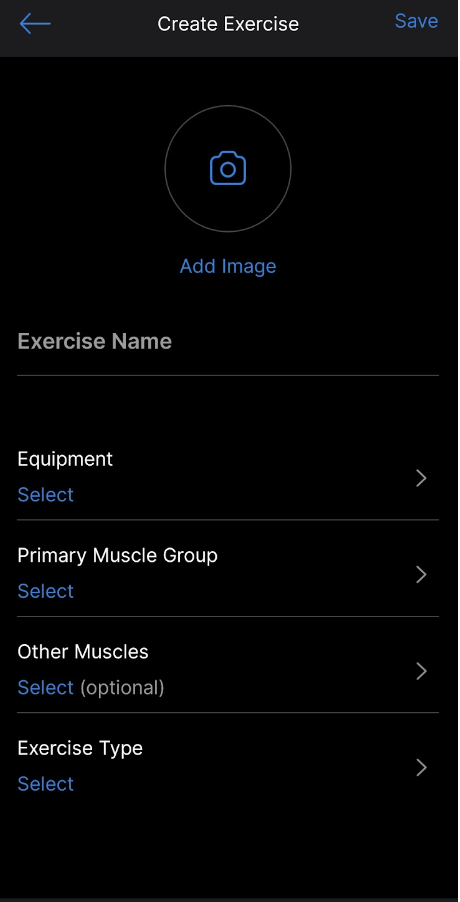
\includegraphics[width=0.4\textwidth]{Figure 7.png}
  \caption{Create exercise page}
\end{figure}

\newpage

This is absolutely an essential feature to add in my application as due to development time constraints, it will not be possible for me to create a comprehensive database of premade exercises. 


\paragraph{Strong}

There is a lot of carryover with the features from each app as they are very similar in a lot of ways. One difference I noticed was the far inferior statistics and analysis features that Strong offers in comparison to Hevy. There are only a few options on the profile tab to add charts that track workouts and exercise weight progressions over time. 

This information is rather surface level and doesn’t really provide much useful insight that would actually help you. Therefore, in my app, I would improve on this and make it more like Hevy. 

The profile system is also a lot less developed than Hevy. This makes sense, since Hevy also doubles as a fitness social media app in many ways, so Strong would have little reason to invest in such features. In my app, I would probably take a similar approach to Strong, as it will operate as a standalone package and users will not be able to interact with each other. 

\begin{figure}[H]
  \centering
  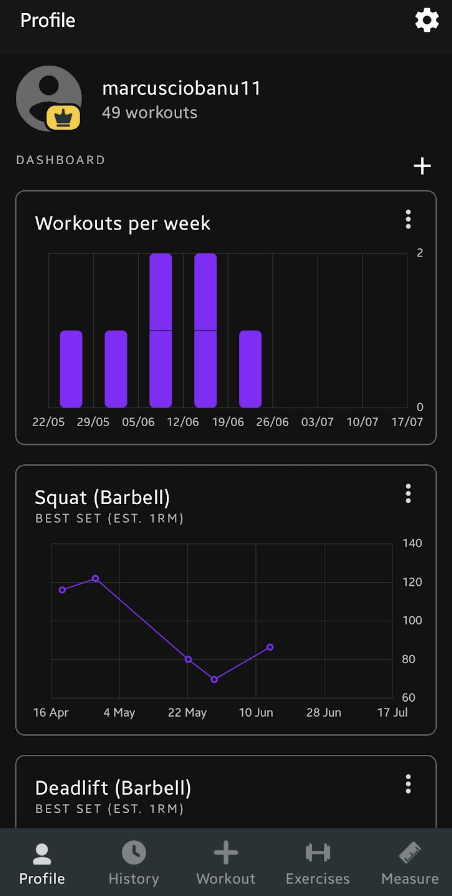
\includegraphics[width=0.4\textwidth]{Figure 8.png}
  \caption{Home page}
\end{figure}

The workout menu also functions in a very similar way to Hevy. However, the template system is far less developed, which is definitely something I would like to improve in my app. I found that the folder and stock template features were very useful so I would like to develop my app in that way. 

Despite this, all the other features are practically identical to Hevy. They function as intended and have utility. The base template of a workout tracker seems to be consistent no matter the developers which is a testament to its effectiveness. A quick start and template system will be integral to the workout tracking system in my application.

\begin{figure}[H]
  \centering
  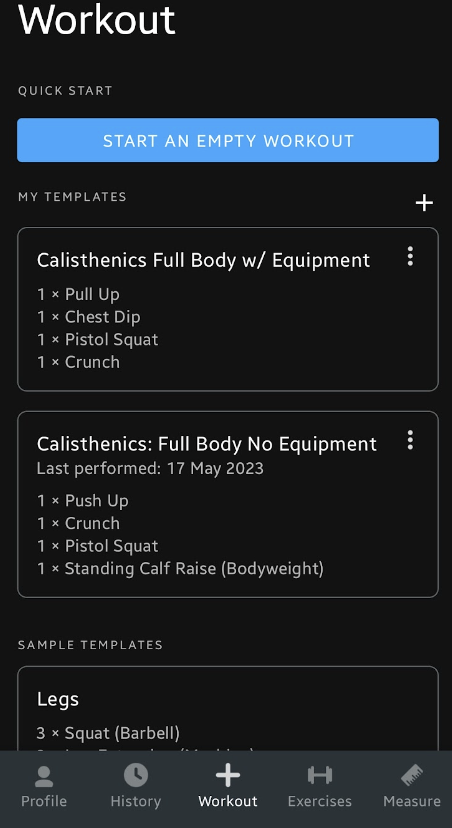
\includegraphics[width=0.4\textwidth]{Figure 9.png}
  \caption{Workout menu}
\end{figure}

The history menu is something that Hevy also has, but the layout in Strong is a lot more minimalist and focuses on showing the most important information. It is also categorised by month so it allows you to block and periodise your training which can certainly have utility for some people.

Overall, where Strong excels is its functional, intuitive and easy to use GUI. Especially for the mobile format, having little to no clutter is something that consumers would definitely appreciate and Strong has done that in a textbook manner. 

It is clear that despite the lack of updates and new features in Strong as compared to Hevy (the Strong developers have given up on the app in many ways), there is still a consistent user base and the reviews remain high. This is a testament to the strong foundation of the app within its core features. 

\paragraph{Summary of features to add}
\begin{itemize}
  \item Quick Start Workout Feature
  \begin{itemize}
    \item This will take the form of an interactive UI element that can be pressed
    \item This is necessary to further tailor my program to the beginner demographic who may not have a rigid routine and would appreciate the ability to start a workout and choose their exercises as they go along
  \end{itemize}
  \item Folder Organisation System
  \begin{itemize}
    \item This will be a niche feature with high utility to ensure that the program also retains good use for more advanced users who may have periodisation blocking and alternate their training regimes.
  \end{itemize} 
  \item Exercise Creation Function
  \begin{itemize}
    \item Essential feature to reduce development and make it so that users can record their workouts no matter the equipment they use or the gym they go to
    \item This will be implemented as its own page that is linked through the workout tracking section.
  \end{itemize}
  \item Statistics Section
  \begin{itemize}
    \item Great feature for both beginners and advanced users alike as it is as detailed and informative as you want it to be and gives useful information to see if you are on the right track
    \item This will have its own dedicated section on the website with multiple pages 
  \end{itemize}
\end{itemize}

\subsubsection{Features of proposed solution}

Key features: 
\begin{itemize}
  \item A workout tracking section with a quick start option and a template creation and selection module with a folder organisation section for training blocking and periodisation
  \item A statistics/analysis section where users can see their muscle group distribution by sets, reps or weight. There should also be graphs to track progressive overload over time. 
  \item A workout history section with a scroll down menu to view all past workouts and the key information from each workout 
\end{itemize}

The listed features above are the most important because they provide the maximum amount of utility to the user. There are many more features I will likely add, but these remain a priority as they are essential to ensuring the program meets the needs of the stakeholders. That being, it is easy to use and intuitive whilst providing useful insight to maximise progress with minimal effort.

\subsubsection{Limitations}

\begin{enumerate}
  \item There will be no user to user connection like Hevy has. In other words, there will be no follow, posting or liking systems and you cannot see the progress of friends etc. This is due to development time constraints.
  \item I will not be able to port this website to mobile formats, so when a mobile browser loads the web app, they will be faced with the desktop layout. This may prove cumbersome for users, but since I am developing on desktop it would make development far easier. Therefore, I will not provide a mobile reformatting again due to time constraints. 
  \item Testing will be limited to desktop. This means that there may be undiscovered bugs that arise when the website is opened on mobile. This, combined with the poor mobile formatting, will make the user experience for this demographic poor, but it is necessary to ensure that the solution is completed on time with the necessary features. 
\end{enumerate}

\subsubsection{Measurable criteria}

\begin{figure}
  \centering
  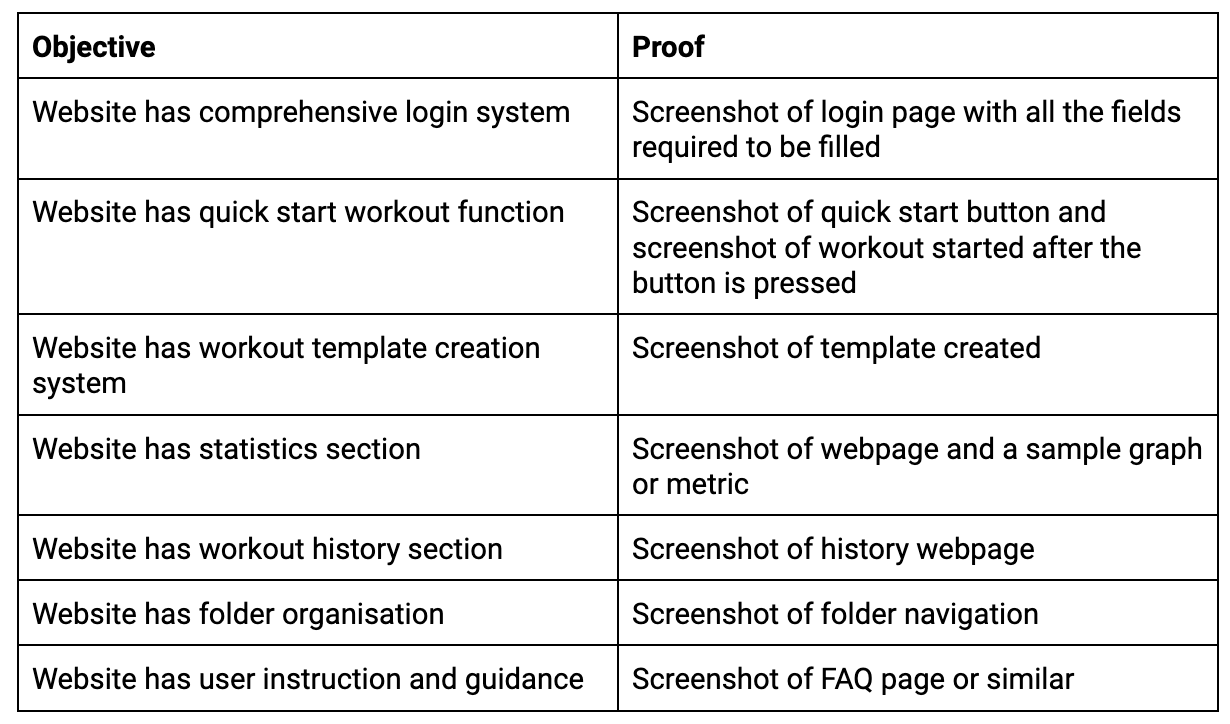
\includegraphics[width=1\textwidth]{Figure 10.png}
  \caption{Measurable criteria}
\end{figure}

\newpage

\subsubsection{Solution requirements}

\begin{itemize}
  \item Users must create or login to an account upon opening website
  \begin{itemize}
    \item Account creation details:
    \begin{itemize}
      \item Name (full)
      \item Username
      \item Email
      \item Password
    \end{itemize}
  \end{itemize}
  \item Users should be able to track and record workouts
  \begin{itemize}
    \item Start a workout by template or quick start
    \item Add exercises (either from the premade database or custom)
    \item Add sets
    \item Add reps 
    \item Specify type of set (drop set, failure set, warm up set, working set)
    \item Be able to view all past workouts
  \end{itemize}
\end{itemize}

These are the core features that will make the web app work, but there are many quality of life features that I will also plan to add. This outlines the bare minimum for it to function as intended with some essential features. Everything else only improves on the user experience in essence. 

In terms of hardware requirements, the device the user is currently on must be able to run a web browser and connect to the internet. They must also have around 1GB of local storage available to leave plenty room for database downloads and caching websites locally.

\section{Design}

\subsection{Problem Decomposition}

As is to be expected with a program of this complexity, there are many moving parts, which would be best tackled by breaking them down into their constituent parts. 

\subsubsection{Features that need to be included}

Following on from the analysis, we need to decide which features will be implemented as a base to provide the essential functionality of the program. Essentially, we are abstracting away any of the extra things which do not form the core of the program. 

\paragraph{Landing Page}

This should be as minimal and bare-bones as possible. The only purpose it serves is letting the user know that they are at the website when they enter the root URL into their browser (now decided to be named europaFitness), and to give them a starting point to enter the actual functionality of the website. 

\paragraph{Registration System} 

This should allow the user to create an account. This will include a username (unique, as it is part of the composite key), email, forename, surname and password. There are a few key requirements for this. Each of the inputs must be validated to ensure they are in the correct format and are unique when needed. Additionally, the password must be hashed before being sent to the database to ensure security. 

\paragraph{Login System}

This naturally follows from the registration system. The login will be made up of the username and password, as that is all that is necessary to uniquely identify a user and make sure it is them who is logging in. 

\paragraph{Dashboard}

This is where the user will be immediately taken to after logging in or registering an account. It will be made up of a sidebar, with the various applications listed on it. At the top of the sidebar will be a website logo, which the user can press to return to the landing  page without ending their session. At the bottom of the sidebar will be a traditional logout button. This sidebar will be on the left of the screen, taking up about 15-20\% of the screen width. This sidebar can also be collapsed even further if the user wishes to focus on the application. 

The rest of the screen will be dedicated to the specific application the user is on.

\paragraph{Home}

The default app selected when entering the dashboard. Simply welcomes the user to the app.

\paragraph{Workout}

This is the core of the web app. It allows a user to quick start a workout on the fly and add in whatever exercises they want from the exercise bank. Then they can add sets to each exercise, specifying weight, number of reps and type of set. The workout will also record how long it took and the date. Once the user is finished, they can submit the entire workout and save it to the database.

\paragraph{History}

Simply allows the user to view a history of workouts done, retrieved from the database, displaying all of the information associated with that workout. It will also allow the user to delete the workout.

\paragraph{Templates}

Allows the user to create templates of workouts consisting of the exercises they want to do. Saves the user time if they follow a regime which involves repeated workouts. On the workout app, the user will then be able to choose whether they want to quick-start a workout or select from their created templates. 

\paragraph{Create Exercise}

Allows the user to create their own exercises and add them to the database and also view all of their added exercises and delete them if they want. 

\paragraph{Error pages}

A set of pages which restrict user access through URL inspection. For example, if a user tries to access the dashboard when they are not logged in, an error screen will be returned informing the user of the error and redirecting them to the login page. 

\subsection{System Design (Problem Modelling)}

\subsubsection{High Level Overview of System Design}

Now that the features that are needed to be implemented are clearly defined, we need to decide how these features are going to be implemented in a broad overview. 

\paragraph{Technologies}

The proposed solution will be a website. Therefore, we need to consider the technologies used for both the client side and server side. I have decided on using HTML, CSS and JS to build the front-end (standard in web-development), and Python for the back-end.

\paragraph{Frameworks}

Various frameworks could be used to help abstract some of the technicalities of many common processes in web-development, both in the front-end and back-end. For the front-end, I will keep it simple and use vanilla HTML, CSS and JavaScript as this is more than sufficient for my needs and gives me extensive control over the design and styling of the website. 

For the back-end, it is essential to use a framework to abstract the tedious tasks of routing HTTP requests and the like. For this I will use Django. Django is a batteries-included, opinionated framework enabling the creation of websites using Python. Since it is batteries-included, it comes with all the packages and dependencies you would likely ever need, all with extensive and detailed documentation. This will make development hassle-free. 

\subsubsection{System Architecture}

Handling the client-server dynamic will be a key consideration when developing the solution. There must be a clear structure to separate the various functionalities of the code. I will be using the MVT (Model, View, Template) architecture to structure my code. See figure 11 for an abstraction of how the MVT architecture functions.

\begin{figure}
  \centering
  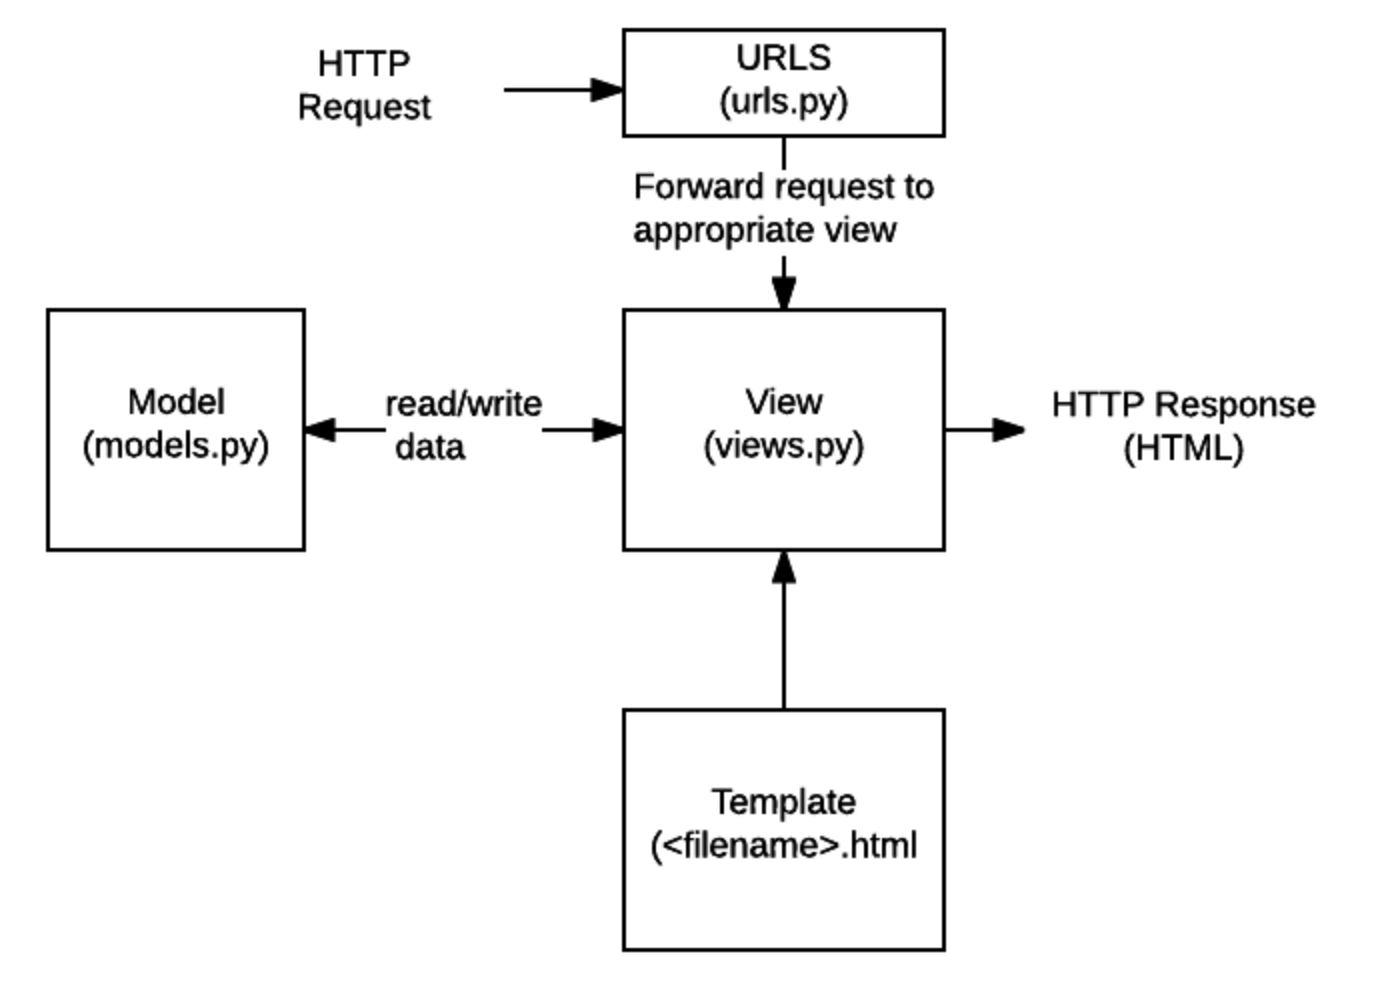
\includegraphics[width=1\textwidth]{Figure 11.png}
  \caption{MVT architecture}
\end{figure}

By nature, the MVT architecture (and by extension, Django itself as a framework) is modular and delegates all tasks to separate modules. As a HTTP request is received by the server, it uses the URL to decide which 'view' function to delegate the task of handling it to. It does this through a 'urls' file, which acts as a traffic warden, directing the flow of the program. The 'urls.py' file in a Django project would map the values of the URL to an appropriate view function. It can also read up to a certain point of a URL and then cut off the part it has already read, handing the rest to a URL file in a certain app that it would be related to, enhancing modularity and maintainability. 

Once it decides which view function to hand it to, the HTTP request is sent to the view. Views control the business logic of a given app. It dictates what you will see when the HTTP response is received, but not necessarily how you will see it. That is, it has no influence over the styling or aesthetics of the rendered page, but does have control over the contents. The view will read the HTTP request and decide what to do next. It may need to gather data from the models. 

Models are an abstraction over traditional databases. In Django, OOP is used to define a model, where each model corresponds to a table in a relational database. The attributes represent fields and the methods define things like initialization of an object, deletion, foreign key relationships and more. This layer of abstraction also provides an extra layer of security, as at no point in the program can a user's inputs ever be mapped directly into an SQL statement. This prevents SQL injection. 

Back to the view function, once the data has been gathered from the models and all associated logic has been calculated, it then delegates the formatting of the HTTP response to the templates. Templates are an extension of traditional HTML. It would be grossly inefficient to manually format each possible HTML file that could be created from a user's inputs. So, we use templates to introduce placeholders (variables) directly into the HTML markup which will then be read and compiled by the template interpreter built into the framework to render the final HTML to be sent in the HTTP response. A important thing to note, the template does not have to be HTML, but for our purposes, it will nearly always be HTML. 

\subsection{Permanent Data Storage}

Underneath the model abstraction, there will still need to be a traditional database for permanent data storage. For this project, I will be using SQLite. It is a lightweight, minimalist SQL database that is suitable for projects of small size. It works best for sites will low concurrent usage which is appropriate for the use case. 

There are a couple of tables that need to be designed. In terms of users, there is a built in module: 'django.contrib.auth' which provides functionality for user creation out of the box. Since there is no use in re-inventing the wheel, I will use this module as it provides hashing of passwords and handling of user registration and logging in forms. As for the workout app, I will design my own relational database. See the ERD in figure 12 for specification of the various fields and relationships of the proposed database. 

\begin{figure}
  \centering
  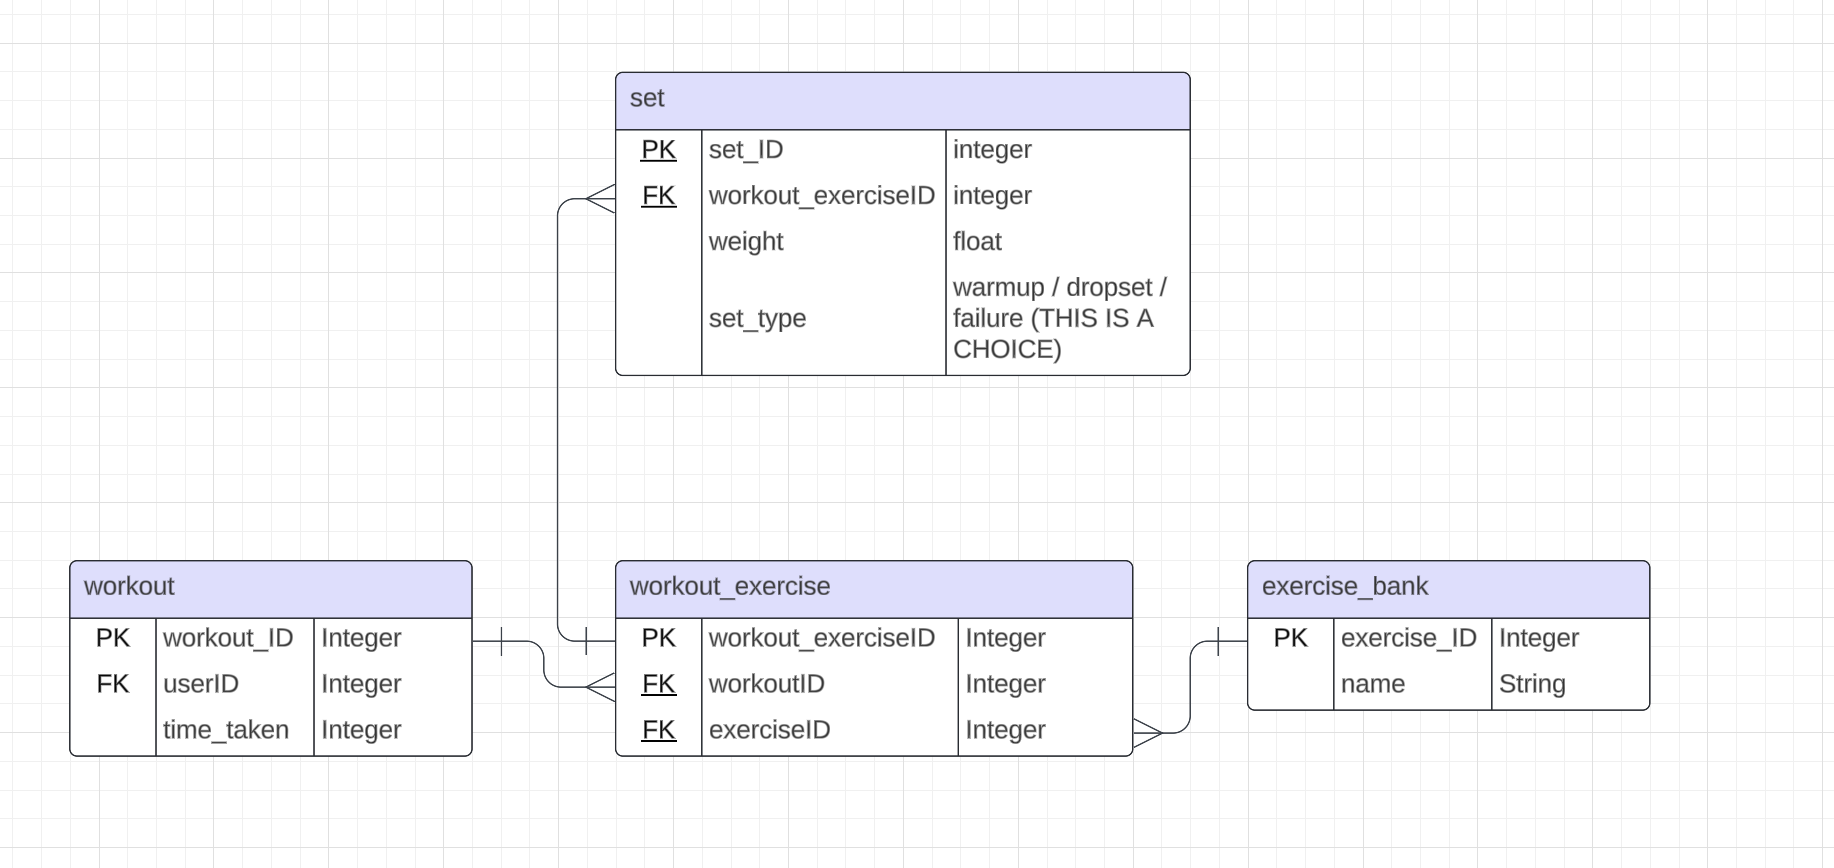
\includegraphics[width=1\textwidth]{Figure 12.png}
  \caption{ERD of database}
\end{figure}

It follows a top down architecture where the workout acts as the parent of the workout\_exercise, which in turn acts as the parent of the set. This is defined through the foreign key relationships. A workout belongs to a user. A workout\_exercise belongs to a workout (the exercise being taken from the exercise\_bank which defines all the created exercises by the user). A set belongs to a workout\_exercise. Many to many relationships have been removed, and the database is normalized. 

\newpage

\subsection{Algorithms}

The proposed solution, when broken down, broadly separates into two main categories: Accounts and Dashboard. These represent Django apps that separate the functionality of the website into two main modules. Accounts handles the face of the website. That is, the landing page and the account creation process/login process. Dashboard is a broad term used to represent all of the different apps identified in the Problem Decomposition: Workout, Exercise Bank, History etc. Below are pseudocode functions for the most important parts of the program. 

\subsubsection{Accounts}

\begin{lstlisting}[caption={Login Page}]
  FUNCTION loginpage(request):
  IF the request is a POST:
      Make a form with the POST data.
      IF the form is okay:
          Get username and password from form.
          Try to log the user in with username and password.
          IF the user is found:
              Log the user in.
              Go to the dashboard home page.
      ENDIF
  ELSE:
      Just show the empty login form.
  ENDIF
  Show the login page with the form.
ENDFUNCTION
\end{lstlisting}

\begin{lstlisting}[caption={Register Page}]
  FUNCTION registerpage(request)
  IF form submitted THEN
    Create form with submitted data
    IF form data is correct THEN
      Save new user
      Log in new user
      Go to dashboard
    ENDIF
  ELSE
    Show empty form
  ENDIF
  Show registration page with form
ENDFUNCTION

\end{lstlisting}

\begin{lstlisting}[caption={CustomUserCreationForm}]
  CLASS CustomUserCreationForm INHERITS UserCreationForm
  SETUP form to use User model and add fields: first name, last name, email
ENDCLASS
\end{lstlisting}

\subsubsection{Dashboard}

\begin{lstlisting}[caption={Exercise Creation view}]
  FUNCTION create(request)
  IF user logged in THEN
    Get user exercises
    IF form submitted THEN
      Create and check form with user data
      IF form correct THEN
        Save exercise
      Reset form after save or if incorrect
    ELSE
      Show new form
    Show page with form and exercises
  ELSE
    Show login error page
  ENDIF
ENDFUNCTION

\end{lstlisting}

\begin{lstlisting}[caption={Exercise deletion view}]
  FUNCTION delete_exercise(request, exercise_id)
  IF user logged in AND form submitted THEN
    Find exercise by id for the logged-in user
    Delete exercise
  Redirect to create page regardless
ENDFUNCTION
\end{lstlisting}

These algorithms do not form the entire solution, as I haven't planned in detail every single function that will make up every app. Arguably, the most complex function will be the workout app main function, as it will involve other modules and classes from throughout the whole function. Therefore, there is an element to iteration to this design, and I will come back to it in the future once I reach the parts that require more design.

\subsection{Identification of Key Variables, Data Structures and Classes}

\subsubsection{Accounts}

Each account is represented by a model class derived from the framework module 'django.contrib.auth'. Each instance of a user class has an ID (integer), username (string), forename, surname and email (all strings). 

Since the default user creation form in Django only includes the username and password, I will need to create a custom user creation form class that inherits from the superclass user creation form. It will then add in the extra fields so that the user can enter their names and email in the form. 

For the registration form, I can use the default registration form as it works perfectly fine for my purposes. Validation is handled by the '.is\_valid()' method that every form inherits from 'django.contrib.auth.models' via the ModelForm superclass. 

\subsubsection{Dashboard}

The main data structure to consider for this is the relational database. Models will need to be created for each table of the database. It will inherit from the superclass 'models.Model', which will handle many of the methods involved with SQL manipulation. For the 'set' model, a 2D array will need to be used to create the inputs for set type, as they can take multiple pre-defined values. 

Various views may need to take in multiple inputs from the HTTP request. Therefore, a dictionary would be the most appropriate data structure to store these. The key value pairs will consist of the variable name and the variable value. Values can then be popped off the dictionary when they need to be called. 

\subsection{Test Plan}

During the iterative development, I will test the functions as I create them to ensure they function correctly, documenting the testing as I go along. Then, post development, I will test the program as a whole to ensure it all works together cohesively. The test data here may not be complete as I haven't planned out all of the functions I will include in full detail yet, so as I develop iteratively I will come back to this and include more functions. 

\subsubsection{Test Data}

\paragraph{Registration Function}

\begin{itemize}
  \item Valid Data:
  \begin{itemize}
    \item Username: User123
    \item Forename: John
    \item Surname: Doe
    \item Email: john.doe@example.com
    \item Password: Password123!
    \item Confirm Password: Password123!
  \end{itemize}
  \item Boundary Data (testing the limits of valid data, such as minimum/maximum lengths):
  \begin{itemize}
    \item Username: Us
    \item Forename: J 
    \item Surname: D
    \item Email: j.d@example.co
    \item Password: Passw0rd!
    \item Confirm Password: Passw0rd!
  \end{itemize}
  \item Erroneous Data (data that should be rejected by the form):
  \begin{itemize}
    \item Username: User@123
    \item Forename: John123
    \item Surname: Doe!
    \item Email: john.doe.com
    \item Password: pass
    \item Confirm Password: pass
  \end{itemize}
  \item Erroneous Data with SQL Injection Attempt (to test for security vulnerabilities):
  \begin{itemize}
    \item Username: 'User123'; DROP TABLE users; --
    \item Forename: John
    \item Surname: Doe
    \item Email: john.doe@example.com
    \item Password: Password123!
    \item Confirm Password: Password123!
  \end{itemize}
\end{itemize}

\paragraph{Login Function}

\begin{itemize}
  \item Valid Data:
  \begin{itemize}
    \item Username: validUser
    \item Password: CorrectP@ssword1
  \end{itemize}
  \item Boundary Data:
  \begin{itemize}
    \item Username: u (minimum length allowed)
    \item Password: P@ssw0rd (minimum complexity)
  \end{itemize}
  \item Erroneous Data:
  \begin{itemize}
    \item Username: invalidUser
    \item Password: WrongPass
  \end{itemize}
  \item Complex Erroneous Data (SQL Injection Test):
  \begin{itemize}
    \item Username: admin' --
    \item Password: anything
  \end{itemize}
\end{itemize}

In each case, the valid data should work and be accepted, creating an account or logging in the user. The boundary data should do the same. The SQL injection attempts should be ineffective due to the abstraction layer provided by the object relational mapper that prevents user inputs from being mapped directly to SQL statements. The erroneous data should be rejected and errors should be returned specifying what needs to be corrected.

\subsection{Usability Features}

\begin{figure}
  \centering
  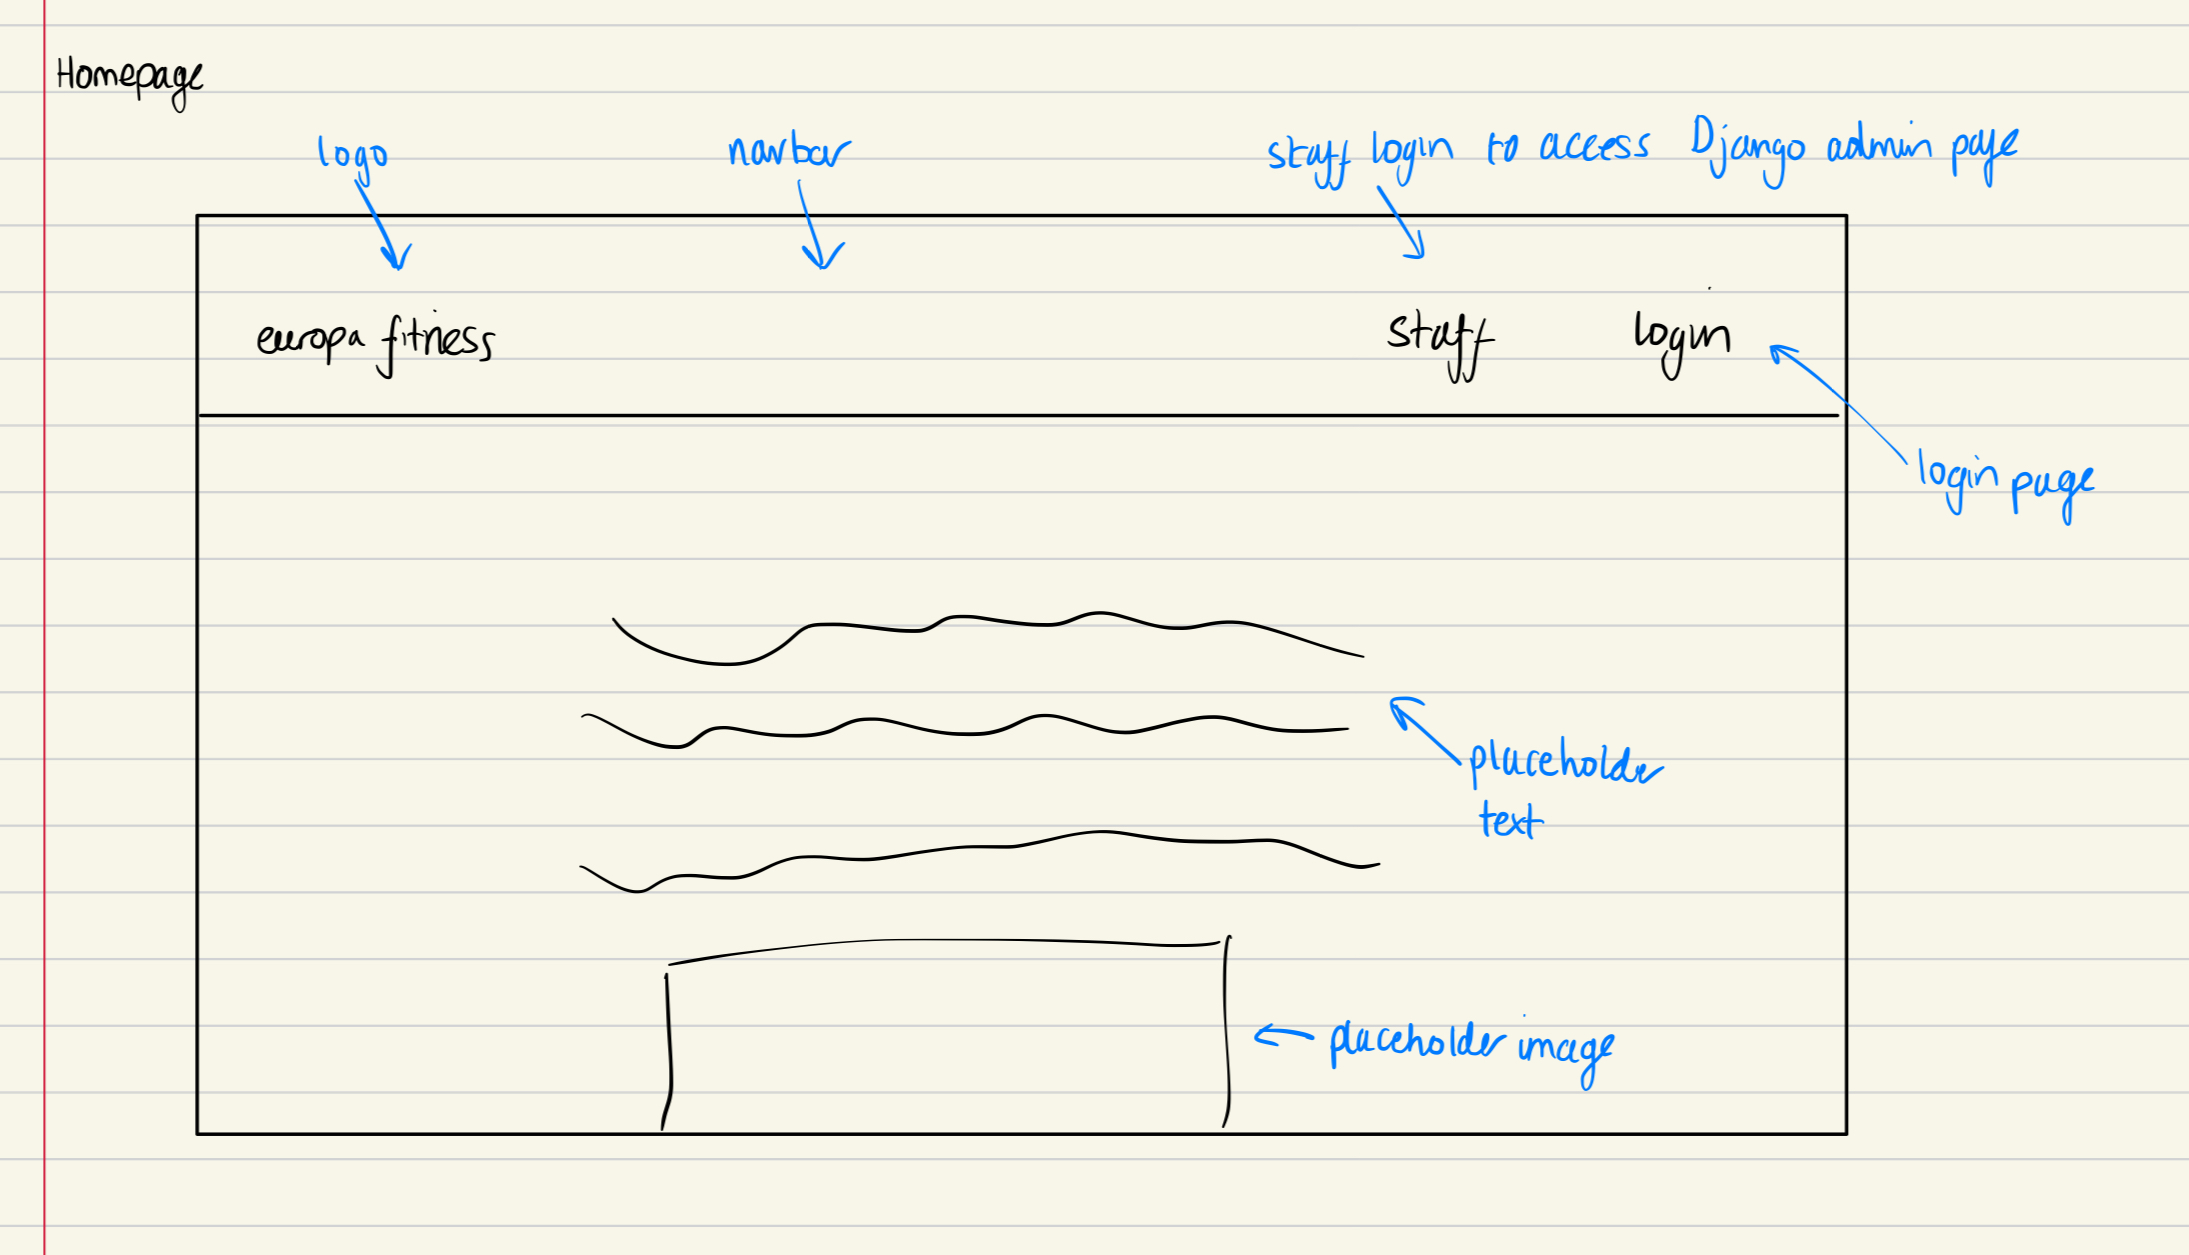
\includegraphics[width=1\textwidth]{Figure 13.jpeg}
  \caption{Mockup of the landing page}
\end{figure}

\begin{figure}
  \centering
  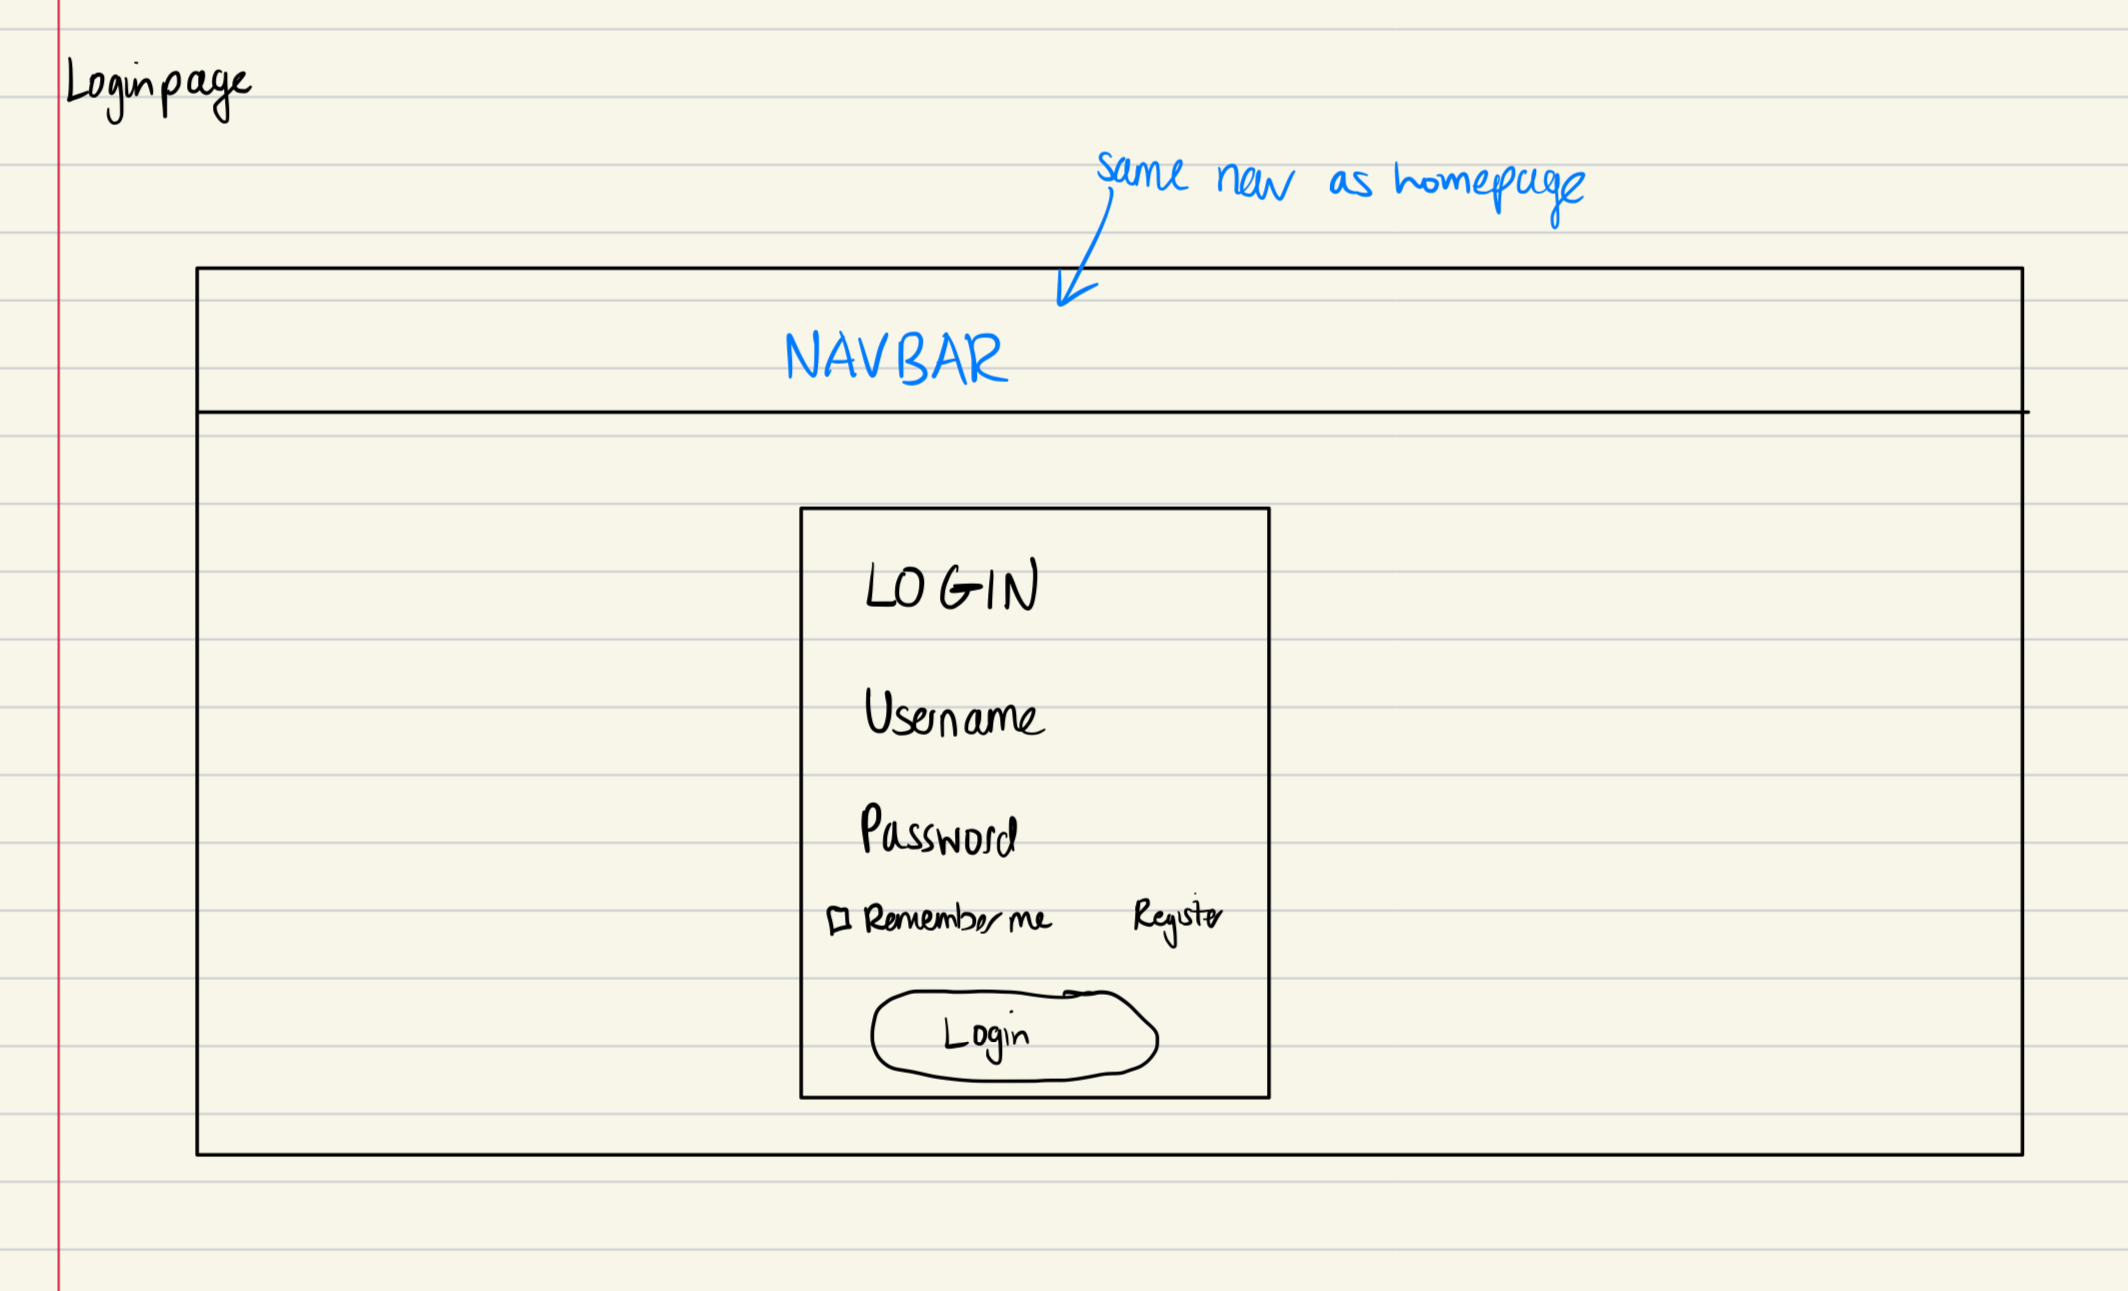
\includegraphics[width=1\textwidth]{Figure 14.jpeg}
  \caption{Mockup of the login page}
\end{figure}

\begin{figure}
  \centering
  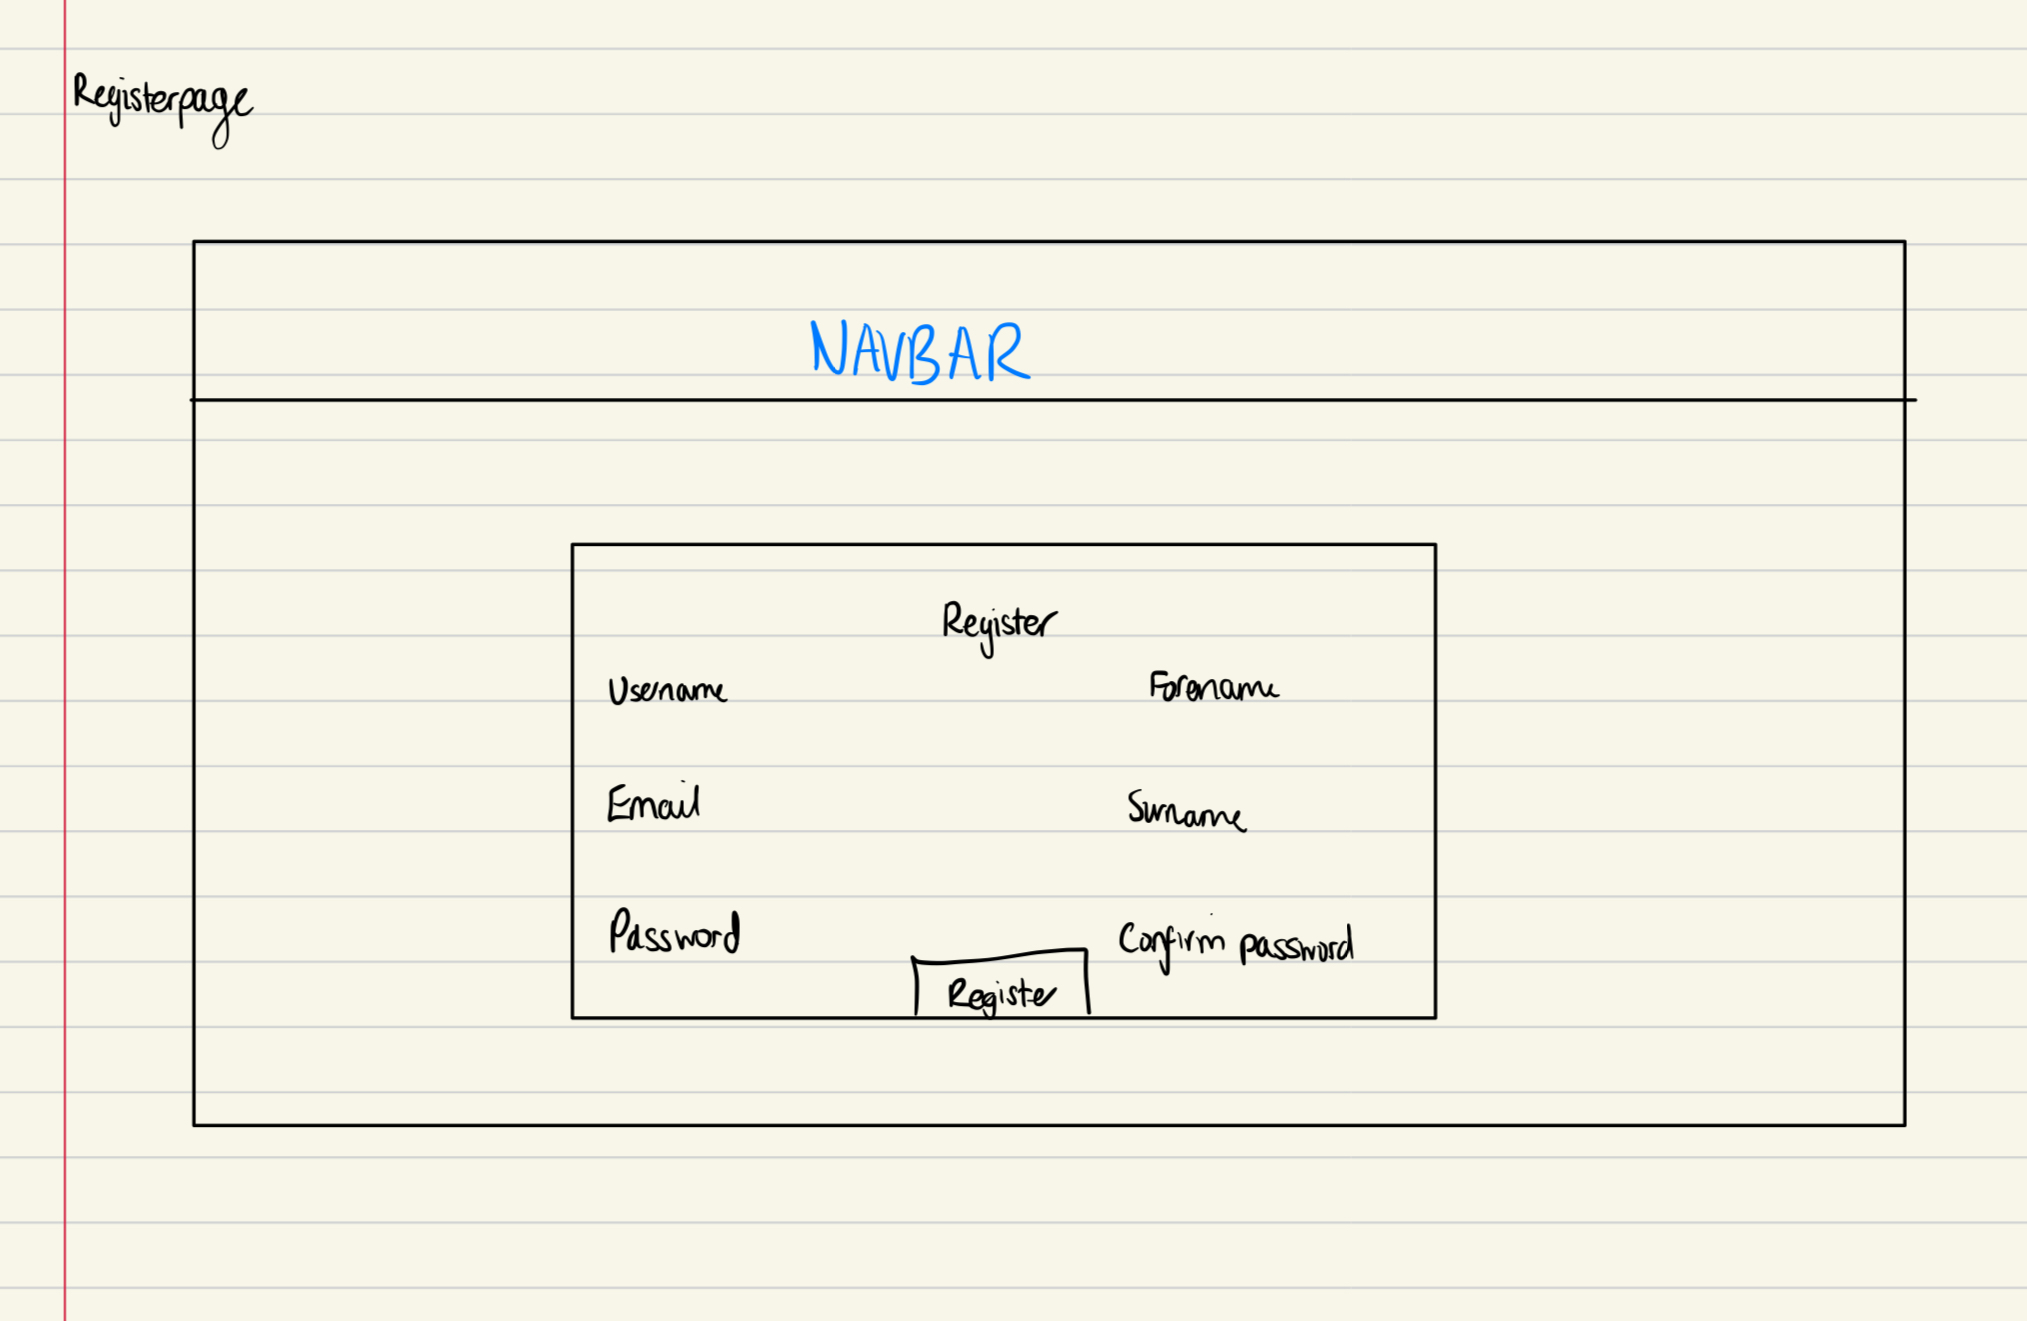
\includegraphics[width=1\textwidth]{Figure 15.jpeg}
  \caption{Mockup of the register page}
\end{figure}

\newpage

\section{Development}

\subsection{Iteration 1}

For the first iteration, I created a basic markup of the landing page with a couple of styles. It was very rudimentary and only served to create an idea of what the website could begin to look like. There was no logic to the page and it was purely made up of static files with no backend code. 

\begin{lstlisting}[caption={index.html}]
  <!DOCTYPE html>
  <html lang="en">
  <head>
    <meta charset="UTF-8">
    <meta name="viewport" content="width=device-width, initial-scale=1.0">
    <title>trackR</title>
    <link rel="stylesheet" href="/css/style.css">
  </head>
  <body>
    <header class="name">
      <a href="landingpage.html">
        trackR
      </a>
    </header>
  
    <nav class="menubar">
      <div>
        <ul>
          <li>
            <a href="#">
              Login
            </a>
          </li>
          <li>
            <a href="#">
              Create Account
            </a>
          </li>
          <li>
            <a href="#">
                <img src="html/img/pfp.png" alt="Profile Picture" width="40">
            </a>
          </li>
        </ul>
      </div>
    </nav>
  
    <div class="placeholder">
      <p>Lorem ipsum dolor sit amet consectetur adipisicing elit. Obcaecati, voluptatibus laborum iure quia neque sint alias repellat eos quod quidem molestiae? Ullam, quibusdam ipsam consequuntur omnis doloribus ea quis beatae
      </p>
    </div>
  
  </body>
  </html>
\end{lstlisting}

The page consisted of a simple nav bar and placeholder for the main portion of the page. It was more or less a less abstracted version of the landing page detailed in the usability features sections, translated into HTML and CSS.

\begin{lstlisting}[caption={style.css}]
  body {
  font-family: Helvetica;
  font-weight: 100;
  background-color: white;
  margin: 0;
}

.name {
  background-color: #19747E;
  padding-left: 10px;
  font-size: 40px;
  font-weight: bolder;
  color: black;
  text-decoration: none;
}

.name a{
  font-size: 40px;
  font-weight: bolder;
  color: black;
  text-decoration: none;
}

.menubar {
  background-color: #A9D6E5;
  overflow: hidden;
  text-align: right;
}

.menubar ul{
  height: 50%;
  margin: auto;
  list-style: none;
}

.menubar li{
  display: inline;
  padding: 25px;
}

.menubar a{
  color: black;
  font-weight: bold;
  text-decoration: none;
}

.menubar li:hover{
  background-color: #19747E;
}

.placeholder {
  padding: 5px 15px;
  line-height: 1.4em;
}
\end{lstlisting}

This rudimentary CSS just made the page bearable to look at. The design was inefficient and inelegant but for a first attempt it would suffice. 

\subsection{Iteration 2}

For this iteration, focus was concentrated on the front-end, working to build up a clean and interactive UI from which I could build the program logic around when it came to the backend. It is also important to note that at this point, I had little to no knowledge of backend development, and was essentially learning as I go along, building up from the basics.

This iteration specifically involved a complete overhaul of the landing page design and a first iteration at the login form and register form. Still, there was no actual functionality and it was purely about the GUI. 

\begin{lstlisting}[caption={landingpage.html}]
  <!DOCTYPE html>
<html lang="en">
<head>
  <meta charset="UTF-8">
  <meta name="viewport" content="width=device-width, initial-scale=1.0">
  <title>Homepage</title>
  <link rel="stylesheet" href="/landingPage/css/landingPage.css">
</head>

<body>

<!-- Content for menubar -->

  <header class="menubar">
    <h2 class="logo">europa fitness</h2>
    <nav class="navigation">
      <a href="landingpage.html">Home</a>
      <button class="loginBtn">Login</button>
    </nav>
  </header>
  
<!-- Content for login form -->

  <div class="wrapper">
    <span class="closeButton">
      <ion-icon name="close-sharp"></ion-icon>
    </span>
    <div class="loginForm">
      <h2>Login</h2>
      <form action="#">
        <div class="inputBox">
          <span class="icon"><ion-icon name="mail-outline"></ion-icon></span>
          <input type="email" required>
          <label>Email</label>
        </div>
        <div class="inputBox">
          <span class="icon"><ion-icon name="key-outline"></ion-icon></span>
          <input type="password" required>
          <label>Password</label>
        </div>
        <div class="rememberForgot">
          <label><input type="checkbox"> Remember me!</label>
          <a href="#">Forgot Password?</a>
        </div>
        <button type="submit" class="btn">Login</button>
        <div class="loginRegister">
          Don't have an account? <a href="#" class="registerLink">Register!</a>
        </div>
      </form>
    </div>
    
<!-- Content for register form -->

    <div class="registerForm">
      <h2>Register</h2>
      <form action="#">
        <div class="inputBox">
          <span class="icon"><ion-icon name="person-outline"></ion-icon></span>
          <input type="text" required>
          <label>Username</label>
        </div>
        <div class="inputBox">
          <span class="icon"><ion-icon name="mail-outline"></ion-icon></span>
          <input type="email" required>
          <label>Email</label>
        </div>
        <div class="inputBox">
          <span class="icon"><ion-icon name="key-outline"></ion-icon></span>
          <input type="password" required>
          <label>Password</label>
        </div>
        <div class="rememberForgot">
          <label><input type="checkbox"> Remember me!</label>
        </div>
        <button type="submit" class="btn">Create Account</button>
        <div class="loginRegister">
          <p>Have an account?</p><a href="#" class="loginLink">Login!</a>
        </div>
      </form>
    </div>
  </div>

<!-- Main bulk content for the landing page -->

  <div class="landingPagePlaceholder">
    <img src="/landingPage/html/img/gymstockimage.jpg" alt="Man lifting weight">
    <h1 id="text1">exercise.</h1>
    <h1 id="text2">diet.</h1>
    <h1 id="text3">all for</h1>
    <h1 id="text4">FREE.</h1>
    <img src="/landingPage/html/img/gymstockimage2.jpg" alt="Rack of weights">
  </div>

<!-- Main script for the landing page -->

<script src="/landingPage/js/landingPage.js"></script>

<!-- Script to access icons used in login and register forms -->

<script type="module" src="https://unpkg.com/ionicons@7.1.0
  /dist/ionicons/ionicons.esm.js"></script>
<script nomodule src="https://unpkg.com/ionicons@7.1.0
  /dist/ionicons/ionicons.js"></script>

</body>

</html>
\end{lstlisting}

The landing page is now essentially completed. It has a fully fledged and stylized navbar, with a login page that pops up when you press the login button. You can also select the register page from the login page. I also used the Ionicons API to utilize their free open source icons within the markup directly.

\begin{lstlisting}[caption={landingpage.css}]
  /* Import the font used for the website. */

@import url('https://fonts.googleapis.com
  /css2?family=Poppins:wght@500&display=swap');

/* Defining the base attributes for any element on the page. */

* {
  margin: 0;
  padding: 0;
  box-sizing: border-box;
  font-family: 'Poppins', sans-serif;
}
body{
  display: flex;
  justify-content: center;
  align-items: center;
  background: black;
  color: white;
}

/* Animations and attributes for the top navigation bar */

.menubar {
  background-color: black;
  position: fixed;
  top: 0;
  left: 0;
  width: 100%;
  padding: 20px 100px;
  box-shadow: 0 10px 8px black;
  display: flex;
  justify-content: space-between;
  align-items: center;
  z-index: 100;
}
.logo {
  font-size: 2em;
  user-select: none;
}
.logo:hover{
  cursor: default;
  color: #afeeee;
  transition-duration: 1s;
}
.logo:not(:hover){
  cursor: default;
  color: white;
  transition-duration: 1s;
}
.navigation a{
  color: white;
  text-decoration: none;
  position: relative;
  font-size: 1.2em;
  margin-left: 2.5em;
}
.navigation a::after{
  content: '';
  position: absolute;
  left: 0;
  bottom: -0.3em;
  width: 0;
  height: 0.15em;
  border-radius: 0.4em;
  background-color: white;
  transition: 0.3s ease-in-out; 
  pointer-events: none; 
}
.navigation a:hover::after, .navigation a:focus::after {
  width: 100%;
}
.navigation .loginBtn {
  font-size: 1.2em;
  width: 5.5em;
  height: 2.5em;
  background: transparent;
  border: 0.15em solid;
  outline: none;
  border-radius: 0.4em;
  cursor: pointer;
  margin-left: 2.5em;
}
.navigation .loginBtn:hover{
  background-color: white;
  border-color: white;
  color: black;
  transition: 0.5s;
}
.navigation .loginBtn:not(:hover){
  background-color: black;
  color: white;
  transition-duration: 0.5s;
}


/* Designing the login form and the register form */

.wrapper{
  position: fixed;
  top: 10em;
  width: 25em;
  height: 35em;
  background: transparent;
  backdrop-filter: blur(20px);
  box-shadow: 0 0 30px rgba(0, 0, 0, 0.5);
  border: 0.15em white solid;
  border-radius: 2em;
  display: flex;
  justify-content: center;
  align-items: center;
  z-index: 10;
  overflow: hidden;
  transform: scale(0);
  transition: transform .5s ease, height .2s ease;
}
.wrapper.popup{
  transform: scale(1);
}
.closeButton{
  position: absolute;
  top: 0;
  right: 0;
  background-color: transparent;
  width: 1.5em;
  height: 1.5em;
  color: white;
  font-size: 2em;
  display: flex;
  align-items: center;
  justify-content: center;
  border-bottom-left-radius: 20px;
  transition-duration: 0.5s;
}
.closeButton:hover {
  cursor: pointer;
  background-color: white;
  color: black;
}
.loginForm,
.registerForm{
  width: 70%;
  padding: 1em;
  background: transparent;
  display: flex;
  flex-direction: column;
  z-index: 11;
}
.wrapper .loginForm{
  transition: .18s ease;
  transform: translateX(0);
}
.wrapper.active .loginForm{
  transition: .18s ease;
  transform: translateX(-30em);
}
.registerForm{
  position: absolute;
  transition: .18s ease;
  transform: translateX(30em);
}
.wrapper.active .registerForm{
  transition: .18s ease;
  transform: translateX(0);
}
.loginForm *,
.registerForm *{
  background: transparent;
}
.loginForm h2,
.registerForm h2{
  font-size: 2em;
  text-align: center;
}
.inputBox{
  position: relative;
  width: 100%;
  height: 3em;
  border-bottom: 0.1em solid white;
  margin: 30px 0;
}
.inputBox label{
  position: absolute;
  top: 50%;
  left: 0.1em;
  transform: translateY(-50%);
  pointer-events: none;
  transition-duration: 0.5s;
}
.inputBox input:focus~label,
.inputBox input:valid~label{
  top: 0.001em;
}
.inputBox input{
  color: white;
  width: 100%;
  height: 100%;
  outline: none;
  border: none;
  font-size: 1em;
  padding: 0.1em 1.5em 0 0;
}
.inputBox .icon{
  position: absolute;
  right: 0.1em;
  top: 0.6em;
  font-size: 1.2em;
}
.rememberForgot{
  display: flex;
  flex-direction: row;
  justify-content: space-between;
  font-size: 0.8em;
  margin: -1.2em 0 2em 0;
}
.rememberForgot label input{
  accent-color: white;
  margin-right: 0.3em;
}
.rememberForgot a{
  color: white;
  text-decoration: none;
}
.rememberForgot a:hover{
  text-decoration: underline;
}
.btn{
  color: white;
  width: 100%;
  margin-bottom: 1.5em;
  padding: 1em;
  border: white solid 0.175em;
  border-radius: 1em;
  cursor: pointer;
  transition-duration: 0.5s;
}
.btn:hover{
  background: white;
  color: black;
}
.loginRegister,
.loginLink{
  width: 100%;
  font-size: 0.9em;
  display: flex;
  flex-direction: row;
  justify-content: space-between;
}
.loginRegister a{
  color: white;
  font-weight: 600;
  text-decoration: none;
}
.loginRegister a:hover{
  text-decoration: underline;
}
.registerForm .loginRegister{
  margin: 0;
  padding: 0;
  width: 100%;
  display: flex;
  flex-direction: row;
  justify-content: space-between;
}
.registerForm .loginRegister p{
  width: 25em;
}

/* Designing the contents of the landing page*/

.landingPagePlaceholder {
  background-color: black;
  display: flex;
  flex-direction: column;
  justify-content: space-around;
  align-items: center;
  user-select: none;
}
.landingPagePlaceholder #text1{
  font-size: 10em;
  background-color: transparent;
  position: absolute;
  z-index: 5;
  bottom: 1.3em;
}
.landingPagePlaceholder #text2{
  font-size: 10em;
  background-color: transparent;
  position: absolute;
  z-index: 5;
}
.landingPagePlaceholder #text3{
  font-size: 10em;
  background-color: transparent;
  position: absolute;
  top: 14em;
  z-index: 5;
}
.landingPagePlaceholder #text4{
  font-size: 10em;
  background-color: transparent;
  position: absolute;
  top: 15em;
  z-index: 5;
}

/* Animating the 'FREE' text to change color when hovering and vice versa. */

.landingPagePlaceholder #text4:hover{
  cursor: default;
  color: #afeeee;
  transition-duration: 1s;
}
.landingPagePlaceholder #text4:not(:hover){
  cursor: default;
  color: white;
  transition-duration: 1s;
}

/* Styling the images on the landing page  */

.landingPagePlaceholder img{
  width: 80%;
  filter: grayscale(100%) brightness(50%);
  margin-left: auto;
  margin-right: auto;
  margin: 5em;
  position: relative;
  top: 5em;
  border-radius: 1em;
}

/* In terms of efficiency and conciseness of code, this is very bloated. I could have accomplished the same thing in a much sleeker way, but for a first attempt it will suffice. */
\end{lstlisting}

Within the CSS i created animations on hover to make the buttons dynamic. The login form activates via a wrapper that makes it visible, applying appropriate styles. 

\begin{lstlisting}[caption={app.js}]
  // Defining constants to make writing easier and more concise

const wrapper = document.querySelector('.wrapper');
const loginLink = document.querySelector('.loginLink');
const registerLink = document.querySelector('.registerLink');
const loginBtn = document.querySelector('.loginBtn');
const closeButton = document.querySelector('.closeButton');

// Detects when user clicks register button and adds class to .wrapper 

registerLink.addEventListener('click', ()=> {
  wrapper.classList.add('active');
});

// Detects when user clicks login button and removes class from .wrapper

loginLink.addEventListener('click', ()=> {
  wrapper.classList.remove('active');
});

// Detects when user clicks on menubar login button and adds popup class to .wrapper

loginBtn.addEventListener('click', ()=> {
  wrapper.classList.add('popup');
  wrapper.classList.remove('active')
});

// Detects when user clicks on cross icon and removes popup class from .wrapper

closeButton.addEventListener('click',()=> {
  wrapper.classList.remove('popup');
});
\end{lstlisting}

Here is the simple JavaScript that adds event listeners to the various buttons in the navbar. It adds active and pop up bars to toggle various CSS classes that will make the login and register pages visible.

\subsection{Iteration 3}

At this point, work began on the backend of the website. I had initialized the Django project, configured the various settings files to suit my needs and instantiated the database (SQLite3), applying the default migrations which set up the administration page (this included the default User and Groups models). As with any framework, there are a lot of boilerplate files created automatically, which, although contain important information, would be unnecessary to document here. For each iteration from now on, only the essential files will be included. 

In terms of the additional functionality I had added at this point, I had routed the URLs to the appropriate views which simply rendered the static pages. I had essentially hooked up the frontend components I had created in the previous iterations to the backend which at this point only serves the correct static files from the HTTP request received when the user enters the URL. 

Here is an overview of the file structure of the project at this point in time. 

\begin{figure}[H] 
  \centering
  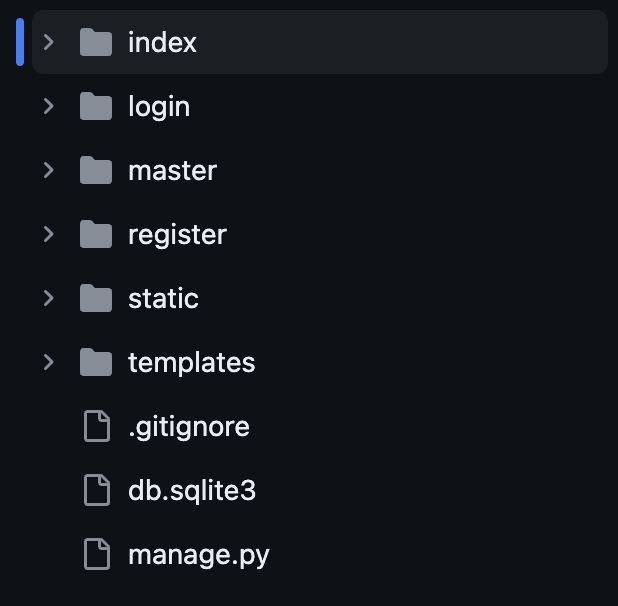
\includegraphics[width=0.5\textwidth]{Figure 16.png}
  \caption{Top level file structure}
\end{figure}

There is quite a lot to unpack here so I will go one by one and explain the functions of each directory. 

\subsubsection{Index, login, master, register}

Each of these directories represent apps. It is a design methodology that places emphasis on modularity. Each app should be fully independent and contain all the necessary components and static files to function independently. The idea is that you can 'plug and play' each app, inserting it into a project and reusing it where needed. Each app consists of a couple of key files. A urls.py, views.py, models.py, forms.py and more depending on the range of functionality required by the app. Even within an app, modularity is encouraged to separate the code into different modules that serve different purposes. 

Within this iteration of the project, there are 4 apps: index, login, master, register. Master is the entry point for the application. When the 'runserver' command is ran from the manage.py script, the project is configured to enter the application from the master application which contains the urls.py for the root URL. It also contains the settings.py file that contains all the configuration for the project. 

\subsubsection{Static}

Within this iteration, since there weren't too many components, I collected all of the static files underneath one directory within the root directory of the project. For production, you would typically create static directories within each of your apps. The static directory is divided into sub-directories for each app. Each contains the necessary static files (that is, CSS, images, JS, audio etc.) needed to be accessed by the various templates. Configured in the settings.py in the master app, the framework knows where to look for these static files as defined when I created the Django project. 

\subsubsection{Templates}

These are the templates for the project. Templates are modified HTML files using the Django templating language which allows context variables to be manipulated within the markup directly. That is, you can dynamically pass in values and perform operations on them such as looping over them. When the view renders the template upon a request for that file, the templating engine built into Django dynamically creates the HTML file to be served to the user depending on the data passed through the view function. It is far more efficient and allows dynamic web pages to be created based on data retrieved from the models. 

\subsubsection{.gitignore}

A file that specifies files to ignore when commiting to the git repository. For example, you wouldnt want to commit sensitive information, encryption keys and the like when creating a respository in production. 

\subsubsection{db.sqlite3}

This is the database for the project. Currently it only has the default user and group models. 

\subsubsection{manage.py}

A python script that allows you to manage the Django project. Also provides functionality for a simple development server that runs on the local host 127.0.0.1 at port 8000. Not suitable for production but entirely sufficient for development purposes. 

\subsubsection{Backend functioality}

\begin{lstlisting}[caption={master/urls.py}]
  from django.contrib import admin
  from django.urls import include, path

  urlpatterns = [
    path('admin/', admin.site.urls),
    path('', include('index.urls')),
    path('login/', include('login.urls')),
    path('register/', include('register.urls')),
  ]
\end{lstlisting}

This is the entry point for the application. When the user enters a URL that corresponds to the domain name of the website, Django will enter from this file to parse the URL and decide which file to serve. When the root URL is followed by 'login/', the login.urls is included. That means that the urls.py from the login app is called and the rest of the URL is cut off and sent to that module for further processing. 

As an example, lets have a look at what happens when the root URL is entered and the URL is sent to index.urls to resolve.

\begin{lstlisting}[caption={index/urls.py}]
from django.urls import path
from . import views

urlpatterns = [
    path('', views.homepage, name='homepage')
]
\end{lstlisting}

As can be seen, the urls.py assigns the root URL to the views.homepage, which is an imported module from the views.py file within the same app. This means that it is now up to the homepage function within the views file to decide what to serve to the user. 

\begin{lstlisting}[caption={index/views.py}]
from django.shortcuts import render


def homepage(request):
    return render(request, 'index.html')
\end{lstlisting}

Here is the very simple views.py file which contains only the homepage function. This function takes in the HTTP request as a parameter (this is conventional, even if the response is static by nature and doesn't require any information from the HTTP request) and returns the rendered HTML template that is index.html. 

\subsubsection{Iterations on the frontend}

Within this iteration, I also made some modifications to the HTML templates. Namely, I modularized them further to separate the landing page, login page and register page into separate templates rendered in different URLs. 

\begin{lstlisting}[caption={templates/index.html}]
<!DOCTYPE html>
<html lang="en">

    <head>
        <meta charset="UTF-8" />
        <meta name="viewport" content="width=device-width, initial-scale=1.0" />
        <title>welcome to europa!</title>
        <link rel="stylesheet" href="" />
    </head>
    <body>
        <!-- Content for menubar -->
        <header class="menubar">
            <h2 class="logo">europa fitness</h2>
            <nav class="navigation">
            <button class="loginBtn">Login</button>
            </nav>
        </header>

        <!-- Main bulk content for the landing page -->

        <div class="landingPagePlaceholder">
            <img src='' alt="Man lifting weights">
            <h1 id="text1">exercise.</h1>
            <h1 id="text2">diet.</h1>
            <h1 id="text3">all for</h1>
            <h1 id="text4">FREE.</h1>
            <img src='' alt="Rack of weights">
        </div>
        <script src=""></script>
    </body>
</html>
\end{lstlisting}

Here you can begin to see some of the templating language in action. At the beginning of the file, all of the static files needed are loaded from their respective directories and template expressions are used to reference the directories of the static files relative to their parent directories. The template engine will convert these to absolute urls upon rendering. This approach is far more maintainable as you can move static files around the project and simply change the STATIC\_FILES\_DIR setting in the settings.py file and the template engine will recognise this and resolve the URLs based on the new settings rather than you having to go through every template and manualy change the URLs.  

\begin{lstlisting}[caption={templates/login.html}]
  <!doctype html>
  <html lang="en">
  
      <head>
          <meta charset="UTF-8">
          <meta name="viewport" content="width=device-width, user-scalable=no, initial-scale=1.0, maximum-scale=1.0, minimum-scale=1.0">
          <meta http-equiv="X-UA-Compatible" content="ie=edge">
          <title>Login to account</title>
          <link rel="stylesheet" href="">
          <link href='https://unpkg.com/boxicons@2.1.4
            /css/boxicons.min.css' rel='stylesheet'>
      </head>
      <body>
          <div class="wrapper">
              <form action="">
                  <h1>Login</h1>
                  <div class="inputbox">
                      <input type="text" placeholder="Username" required>
                      <i class='bx bxs-user'></i>
                  </div>
                  <div class="inputbox">
                      <input type="password" placeholder="Password" required>
                      <i class='bx bxs-key'></i>
                  </div>
                  <div class="rememberForgot">
                      <label><input type="checkbox"> Remember me?</label>
                      <a href="#">Forgot Password?</a>
                  </div>
                  <button type="submit" class="button">Login</button>
                  <div class="registerLink">
                      <p>Don't have an account? <a href="../register">Register</a></p>
                  </div>
              </form>
          </div>
      </body>
  </html>
\end{lstlisting}

\begin{lstlisting}[caption={templates/register.html}]
  <!doctype html>
  <html lang="en">
  
  <head>
      <meta charset="UTF-8">
      <meta name="viewport" content="width=device-width, user-scalable=no, initial-scale=1.0, maximum-scale=1.0, minimum-scale=1.0">
      <meta http-equiv="X-UA-Compatible" content="ie=edge">
      <title>Register for an account</title>
      <link rel="stylesheet" href="">
      <link href='https://unpkg.com/boxicons@2.1.4/css/boxicons.min.css' rel='stylesheet'>
  
  </head>
  <body>
      <div class="wrapper">
          <form action="">
              <h1>Registration</h1>
              <div class="inputbox">
                  <div class="inputfield">
                      <input type="text" placeholder="Full Name" required>
                      <i class='bx bxs-user'></i>
                  </div>
                  <div class="inputfield">
                      <input type="text" placeholder="Username" required>
                      <i class='bx bxs-user'></i>
                  </div>
              </div>
              <div class="inputbox">
                  <div class="inputfield">
                      <input type="email" placeholder="Email" required>
                      <i class='bx bxs-envelope'></i>
                  </div>
                  <div class="inputfield">
                      <input type="number" placeholder="Phone Number" required>
                      <i class='bx bxs-phone'></i>
                  </div>
              </div>
              <div class="inputbox">
                  <div class="inputfield">
                      <input type="password" placeholder="Password" required>
                      <i class='bx bxs-key'></i>
                  </div>
                  <div class="inputfield">
                      <input type="password" placeholder="Confirm Password" required>
                      <i class='bx bxs-key'></i>
                  </div>
              </div>
              <label>Already have an account? <a href="../login">Click here!</a></label>
              <button type="submit" class="button">Register</button>
          </form>
      </div>
  </body>
  </html>
\end{lstlisting}

It's a similar story with these other 2 templates. Static files are collected and served and the template is rendered and sent to the user when the appropriate URL is accessed. That about sums up the backend functionality added within this iteration. 
\end{document}

